% Lines starting with a percent sign (%) are comments. LaTeX will 
% not process those lines. Similarly, everything after a percent 
% sign in a line is considered a comment. To produce a percent sign
% in the output, write \% (backslash followed by the percent sign). 
% ==================================================================
% Usage instructions:
% ------------------------------------------------------------------
% The file is heavily commented so that you know what the various
% commands do. Feel free to remove any comments you don't need from
% your own copy. When redistributing the example thesis file, please
% retain all the comments for the benefit of other thesis writers! 
% ==================================================================
% Compilation instructions: 
% ------------------------------------------------------------------
% Use pdflatex to compile! Input images are expected as PDF files.
% Example compilation:
% ------------------------------------------------------------------
% > pdflatex thesis-example.tex
% > bibtex thesis-example
% > pdflatex thesis-example.tex
% > pdflatex thesis-example.tex
% ------------------------------------------------------------------
% You need to run pdflatex multiple times so that all the cross-references
% are fixed. pdflatex will tell you if you need to re-run it (a warning
% will be issued)  
% ------------------------------------------------------------------
% Compilation has been tested to work in ukk.cs.hut.fi and kosh.hut.fi
% - if you have problems of missing .sty -files, then the local LaTeX
% environment does not have all the required packages installed.
% For example, when compiling in vipunen.hut.fi, you get an error that
% tikz.sty is missing - in this case you must either compile somewhere
% else, or you cannot use TikZ graphics in your thesis and must therefore
% remove or comment out the tikz package and all the tikz definitions. 
% ------------------------------------------------------------------

% General information
% ==================================================================
% Package documentation:
% 
% The comments often refer to package documentation. (Almost) all LaTeX
% packages have documentation accompanying them, so you can read the
% package documentation for further information. When a package 'xxx' is
% installed to your local LaTeX environment (the document compiles
% when you have \usepackage{xxx} and LaTeX does not complain), you can 
% find the documentation somewhere in the local LaTeX texmf directory
% hierarchy. In ukk.cs.hut.fi, this is /usr/texlive/2008/texmf-dist,
% and the documentation for the titlesec package (for example) can be 
% found at /usr/texlive/2008/texmf-dist/doc/latex/titlesec/titlesec.pdf.
% Most often the documentation is located as a PDF file in 
% /usr/texlive/2008/texmf-dist/doc/latex/xxx, where xxx is the package name; 
% however, documentation for TikZ is in
% /usr/texlive/2008/texmf-dist/doc/latex/generic/pgf/pgfmanual.pdf
% (this is because TikZ is a front-end for PGF, which is meant to be a 
% generic portable graphics format for LaTeX).
% You can try to look for the package manual using the ``find'' shell
% command in Linux machines; the find databases are up-to-date at least
% in ukk.cs.hut.fi. Just type ``find xxx'', where xxx is the package
% name, and you should find a documentation file.
% Note that in some packages, the documentation is in the DVI file
% format. In this case, you can copy the DVI file to your home directory,
% and convert it to PDF with the dvipdfm command (or you can read the
% DVI file directly with a DVI viewer).
% 
% If you can't find the documentation for a package, just try Googling
% for ``latex packagename''; most often you can get a direct link to the
% package manual in PDF format.
% ------------------------------------------------------------------


% Document class for the thesis is report
% ------------------------------------------------------------------
% You can change this but do so at your own risk - it may break other things.
% Note that the option pdftext is used for pdflatex; there is no
% pdflatex option. 
% ------------------------------------------------------------------
\documentclass[12pt,a4paper,oneside,pdftex,dvipsnames]{report}

% The input files (tex files) are encoded with the latin-1 encoding 
% (ISO-8859-1 works). Change the latin1-option if you use UTF8 
% (at some point LaTeX did not work with UTF8, but I'm not sure
% what the current situation is) 
\usepackage[latin1]{inputenc}
% OT1 font encoding seems to work better than T1. Check the rendered
% PDF file to see if the fonts are encoded properly as vectors (instead
% of rendered bitmaps). You can do this by zooming very close to any letter 
% - if the letter is shown pixelated, you should change this setting 
% (try commenting out the entire line, for example).  
\usepackage[OT1]{fontenc}
% The babel package provides hyphenating instructions for LaTeX. Give
% the languages you wish to use in your thesis as options to the babel
% package (as shown below). You can remove any language you are not
% going to use.
% Examples of valid language codes: english (or USenglish), british, 
% finnish, swedish; and so on.
\usepackage[english]{babel}

\usepackage{lmodern}    
\usepackage{ifthen} 
% Font selection
% ------------------------------------------------------------------
% The default LaTeX font is a very good font for rendering your 
% thesis. It is a very professional font, which will always be 
% accepted. 
% If you, however, wish to spicen up your thesis, you can try out
% these font variants by uncommenting one of the following lines
% (or by finding another font package). The fonts shown here are 
% all fonts that you could use in your thesis (not too silly). 
% Changing the font causes the layouts to shift a bit; you many
% need to manually adjust some layouts. Check the warning messages
% LaTeX gives you.
% ------------------------------------------------------------------
% To find another font, check out the font catalogue from
% http://www.tug.dk/FontCatalogue/mathfonts.html
% This link points to the list of fonts that support maths, but
% that's a fairly important point for master's theses.
% ------------------------------------------------------------------
% <rant>
% Remember, there is no excuse to use Comic Sans, ever, in any
% situation! (Well, maybe in speech bubbles in comics, but there 
% are better options for those too)
% </rant>

% \usepackage{palatino}
% \usepackage{tgpagella}



% Optional packages
% ------------------------------------------------------------------
% Select those packages that you need for your thesis. You may delete
% or comment the rest.

% Natbib allows you to select the format of the bibliography references.
% The first example uses numbered citations: 
\usepackage[square,sort&compress,numbers]{natbib}
% The second example uses author-year citations.
% If you use author-year citations, change the bibliography style (below); 
% acm style does not work with author-year citations.
% Also, you should use \citet (cite in text) when you wish to refer
% to the author directly (\citet{blaablaa} said blaa blaa), and 
% \citep when you wish to refer similarly than with numbered citations
% (It has been said that blaa blaa~\citep{blaablaa}).
% \usepackage[square]{natbib}

% The alltt package provides an all-teletype environment that acts
% like verbatim but you can use LaTeX commands in it. Uncomment if 
% you want to use this environment. 
% \usepackage{alltt}



% Verbatim provides a standard teletype environment that renderes
% the text exactly as written in the tex file. Useful for code
% snippets (although you can also use the listings package to get
% automatic code formatting). 
\usepackage{verbatim}

% The listing package provides automatic code formatting utilities
% so that you can copy-paste code examples and have them rendered
% nicely. See the package documentation for details.
% \usepackage{listings}

% The fancuvrb package provides fancier verbatim environments 
% (you can, for example, put borders around the verbatim text area
% and so on). See package for details.
% \usepackage{fancyvrb}

% Supertabular provides a tabular environment that can span multiple 
% pages. 
%\usepackage{supertabular}
% Longtable provides a tabular environment that can span multiple 
% pages. This is used in the example acronyms file. 
\usepackage{longtable}

%\usepackage{algorithm}
%\usepackage{algpseudocode}
\usepackage{algorithm2e}
% The fancyhdr package allows you to set your the page headers 
% manually, and allows you to add separator lines and so on. 
% Check the package documentation. 
% \usepackage{fancyhdr}

% Subfigure package allows you to use subfigures (i.e. many subfigures
% within one figure environment). These can have different labels and
% they are numbered automatically. Check the package documentation. 
\usepackage{subfigure}

% The titlesec package can be used to alter the look of the titles 
% of sections, chapters, and so on. This example uses the ``medium'' 
% package option which sets the titles to a medium size, making them
% a bit smaller than what is the default. You can fine-tune the 
% title fonts and sizes by using the package options. See the package
% documentation.
\usepackage[medium]{titlesec}

% The TikZ package allows you to create professional technical figures.
% The learning curve is quite steep, but it is definitely worth it if 
% you wish to have really good-looking technical figures. 
\usepackage{tikz}
% You also need to specify which TikZ libraries you use
\usetikzlibrary{positioning}
\usetikzlibrary{calc}
\usetikzlibrary{arrows}
\usetikzlibrary{decorations.pathmorphing,decorations.markings}
\usetikzlibrary{shapes}
\usetikzlibrary{patterns}

%display grid for preview
%\usepackage[grid]{eso-pic}
%\usepackage{kantlipsum}
% The aalto-thesis package provides typesetting instructions for the
% standard master's thesis parts (abstracts, front page, and so on)
% Load this package second-to-last, just before the hyperref package.
% Options that you can use: 
%   mydraft - renders the thesis in draft mode. 
%             Do not use for the final version. 
%   doublenumbering - [optional] number the first pages of the thesis
%                     with roman numerals (i, ii, iii, ...); and start
%                     arabic numbering (1, 2, 3, ...) only on the 
%                     first page of the first chapter
%   twoinstructors  - changes the title of instructors to plural form
%   twosupervisors  - changes the title of supervisors to plural form
\usepackage[twosupervisors]{aalto-thesis}
%\usepackage[mydraft,doublenumbering]{aalto-thesis}
%\usepackage{aalto-thesis}



% Hyperref
% ------------------------------------------------------------------
% Hyperref creates links from URLs, for references, and creates a
% TOC in the PDF file.
% This package must be the last one you include, because it has
% compatibility issues with many other packages and it fixes
% those issues when it is loaded.   
%\RequirePackage[pdftex]{hyperref}
\RequirePackage[pdfa]{hyperref}
% Setup hyperref so that links are clickable but do not look 
% different

\usepackage[]{xcolor}
%\newcommand\myshade{85}
%\colorlet{mylinkcolor}{violet}
%\colorlet{mycitecolor}{yellow-orange}
%\colorlet{myurlcolor}{Aquamarine}

\hypersetup{colorlinks=true, citecolor=YellowOrange, linkcolor=violet, urlcolor=TealBlue}
\hypersetup{pdfborder={0 0 0}}
\hypersetup{bookmarksnumbered=true}
% The following line suggests the PDF reader that it should show the 
% first level of bookmarks opened in the hierarchical bookmark view. 
\hypersetup{bookmarksopen=true,bookmarksopenlevel=1}
% Hyperref can also set up the PDF metadata fields. These are
% set a bit later on, after the thesis setup.   


\usepackage[toc,acronym, nonumberlist, nogroupskip]{glossaries}

\makeglossaries
% Thesis setup
% ==================================================================
% Change these to fit your own thesis.
% \COMMAND always refers to the English version;
% \FCOMMAND refers to the Finnish version; and
% \SCOMMAND refers to the Swedish version.
% You may comment/remove those language variants that you do not use
% (but then you must not include the abstracts for that language)
% ------------------------------------------------------------------
% If you do not find the command for a text that is shown in the cover page or
% in the abstract texts, check the aalto-thesis.sty file and locate the text
% from there. 
% All the texts are configured in language-specific blocks (lots of commands
% that look like this: \renewcommand{\ATCITY}{Espoo}.
% You can just fix the texts there. Just remember to check all the language
% variants you use (they are all there in the same place). 
% ------------------------------------------------------------------
\newcommand{\TITLE}{Large Scale Speech Recognition}
\newcommand{\SUBTITLE}{with Deep Learning}
\newcommand{\DATE}{September 30, 2021}

\newcommand{\FTITLE}{Large Scale Speech Recognition}
\newcommand{\FSUBTITLE}{with Deep Learning}
% Supervisors and instructors
% ------------------------------------------------------------------
% Usually thesis have one supervisor and one advisor. Sometimes you
% may have two advisors and, in double degree
% programs, you may have two supervisors. 
% If you have two supervisors, write both names here, separate them with a 
% double-backslash (see below for an example)
% Also remember to add the package option ``twosupervisors'' or
% ``twoinstructors'' to the aalto-thesis package (aalto-thesis.sty
% file line 72), so that the titles are in plural.
% Example of one supervisor:
%\newcommand{\SUPERVISOR}{Professor Antti Ylä-Jääski}
%\newcommand{\FSUPERVISOR}{Professori Antti Ylä-Jääski}
%\newcommand{\SSUPERVISOR}{Professor Antti Ylä-Jääski}
% Example of twosupervisors:
\newcommand{\SUPERVISOR}{Prof. Mikko Kurimo\\
  Prof. Sebastian M\"oller}

% If you have only one instructor, just write one name here
\newcommand{\INSTRUCTOR}{Aku Rouhe M.Sc., Aalto University}
\newcommand{\FINSTRUCTOR}{Aku Rouhe M.Sc., Aalto University}
% If you have two instructors, separate them with \\ to create linefeeds
% \newcommand{\INSTRUCTOR}{Oili Ohjaaja M.Sc. (Tech.)\\
%  Elli Opas M.Sc. (Tech)}
%\newcommand{\FINSTRUCTOR}{Diplomi-insinööri Oili Ohjaaja\\
%  Diplomi-insinööri Elli Opas}
%\newcommand{\SINSTRUCTOR}{Diplomingenjör Oili Ohjaaja\\
%  Diplomingenjör Elli Opas}

% If you have two supervisors, it is common to write the schools
% of the supervisors in the cover page. If the following command is defined,
% then the supervisor names shown here are printed in the cover page. Otherwise,
% the supervisor names defined above are used.
\newcommand{\COVERSUPERVISOR}{Prof. Mikko Kurimo, Aalto University\\
  Prof. Sebastian M\"oller, TU Berlin}

% The same option is for the instructors, if you have multiple instructors.
% \newcommand{\COVERINSTRUCTOR}{Oili Ohjaaja M.Sc. (Tech.), Aalto University\\
%  Elli Opas M.Sc. (Tech), Aalto SCI}


% Other stuff
% ------------------------------------------------------------------
\newcommand{\PROFESSORSHIP}{Data Science}
% Professorship code is the same in all languages
\newcommand{\PROFCODE}{SCI3095}
\newcommand{\FPROFESSORSHIP}{Datenwissenschaft}

\newcommand{\MINOR}{Innovation \& Entrepreneurship}
\newcommand{\FMINOR}{Innovation \& Unternehmertum}

\newcommand{\KEYWORDS}{Speech Recognition, Deep Learning, Large-scale, Multi-GPU training, Hogwild, Data Parallel, Attention Models, Recurrent Neural Networks, SpeechBrain, PyTorch}
\newcommand{\FKEYWORDS}{Spracherkennung, Deep Learning, gro\ss{} angelegt, Multi-GPU training, Hogwild, Datenparallel, Aufmerksamkeitsmodelle, wiederkehrende neuronale Netze, SpeechBrain, PyTorch}
%\newcommand{\FKEYWORDS}{aineistot, aitta, akustiikka, Alankomaat,
%aluerakentaminen, aapinen, ankka, aasinsilta}
%\newcommand{\SKEYWORDS}{omsättning, kassaflöde, värdepappersmarknadslagen,
%yrkesutövare, intresseföretag, verifieringskedja}
\newcommand{\LANGUAGE}{English}
\newcommand{\FLANGUAGE}{Englisch}

% Author is the same for all languages
\newcommand{\AUTHOR}{Anand Umashankar}


% Currently the English versions are used for the PDF file metadata
% Set the PDF title
\hypersetup{pdftitle={\TITLE\ \SUBTITLE}}
% Set the PDF author
\hypersetup{pdfauthor={\AUTHOR}}
% Set the PDF keywords
\hypersetup{pdfkeywords={\KEYWORDS}}
% Set the PDF subject
\hypersetup{pdfsubject={Master's Thesis}}


% Layout settings
% ------------------------------------------------------------------

% When you write in English, you should use the standard LaTeX 
% paragraph formatting: paragraphs are indented, and there is no 
% space between paragraphs.
% When writing in Finnish, we often use no indentation in the
% beginning of the paragraph, and there is some space between the 
% paragraphs. 

% If you write your thesis Finnish, uncomment these lines; if 
% you write in English, leave these lines commented! 
% \setlength{\parindent}{0pt}
% \setlength{\parskip}{1ex}

% Use this to control how much space there is between each line of text.
% 1 is normal (no extra space), 1.3 is about one-half more space, and
% 1.6 is about double line spacing.  
% \linespread{1} % This is the default
% \linespread{1.3}

% Bibliography style
% acm style gives you a basic reference style. It works only with numbered
% references.
\bibliographystyle{acm}
% Plainnat is a plain style that works with both numbered and name citations.
% \bibliographystyle{plainnat}


% Extra hyphenation settings
% ------------------------------------------------------------------
% You can list here all the files that are not hyphenated correctly.
% You can provide many \hyphenation commands and/or separate each word
% with a space inside a single command. Put hyphens in the places where
% a word can be hyphenated.
% Note that (by default) LaTeX will not hyphenate words that already
% have a hyphen in them (for example, if you write ``structure-modification 
% operation'', the word structure-modification will never be hyphenated).
% You need a special package to hyphenate those words.
\hyphenation{di-gi-taa-li-sta yksi-suun-tai-sta}

\usepackage{tcolorbox}
\newtcbox{\inlinecode}{on line, boxrule=0pt, boxsep=0pt, top=2pt, left=2pt, bottom=2pt, right=2pt, colback=gray!15, colframe=white, fontupper={\ttfamily}}

% The preamble ends here, and the document begins. 
% Place all formatting commands and such before this line.
% ------------------------------------------------------------------
\begin{document}
% This command adds a PDF bookmark to the cover page. You may leave
% it out if you don't like it...
\pdfbookmark[0]{Cover page}{bookmark.0.cover}
% This command is defined in aalto-thesis.sty. It controls the page 
% numbering based on whether the doublenumbering option is specified
\startcoverpage

% Cover page
% ------------------------------------------------------------------
% Options: finnish, english, and swedish
% These control in which language the cover-page information is shown
\coverpage{english}

\cleardoublepage
Placeholder 
\newpage
\cleardoublepage
\addcontentsline{toc}{chapter}{Acknowledgements}
\chapter*{Acknowledgements}

I thank the 
\cleardoublepage
% Abstracts
% ------------------------------------------------------------------
% Include an abstract in the language that the thesis is written in,
% and if your native language is Finnish or Swedish, one in that language.

% Abstract in English
% ------------------------------------------------------------------
%\addcontentsline{toc}{chapter}{Abstract in English}
\thesisabstract{english}{
Automatic Speech Recognition (ASR) is the task of converting speech signal into text. This thesis focuses on scaling up the training of end to end speech recognition neural networks to enable using large datasets to train them. The main focus of the thesis is to provide guidelines for building a pipeline to increase efficiency in data storing, data loading and training. 

This work uses a dataset with around 26,000 hours that is relatively new for speech to text experiments. The experiments start with exploring the steps taken to make this dataset usable for speech recognition. Then, two types of distributed training algorithms, synchronous and asynchronous training, are applied which enables the usage of multiple GPUs for stochastic gradient descent. This reduces the time taken for models to converge and comparison of the different methods show that for the experiment setup employed in this work, synchronous training provides the best word error rate of 10.87\% and this run converged in 32 hours using 4 GPUs in parallel. 
}

%\addcontentsline{toc}{chapter}{Abstract in German}
% Abstract in Finnish
% ------------------------------------------------------------------
\thesisabstract{german}{
Automatische Spracherkennung (ASR) ist die Aufgabe der Umwandlung von Sprachsignalen in Text. Diese Arbeit befasst sich mit der Skalierung des Trainings von neuronalen Netzen f\"ur die End-to-End-Spracherkennung, um die Verwendung gro\ss{}er Datens\"atze zum Training zu erm\"oglichen. Der Schwerpunkt der Arbeit liegt auf der Erstellung von Richtlinien f\"ur den Aufbau einer Pipeline zur Steigerung der Effizienz bei der Datenspeicherung, dem Laden von Daten und dem Training. 

In dieser Arbeit wird ein Datensatz mit etwa 26.000 Stunden verwendet, der relativ neu f\"ur Experimente mit Sprache zu Text ist. Die Experimente beginnen mit der Untersuchung der Schritte, die unternommen wurden, um diesen Datensatz f\"ur die Spracherkennung nutzbar zu machen. Dann werden zwei Arten von verteilten Trainingsalgorithmen, synchrones und asynchrones Training, angewandt, die die Verwendung mehrerer GPUs f\"ur stochastischen Gradientenabstieg erm\"oglichen. Dadurch wird die Konvergenzzeit der Modelle verk\"urzt. Der Vergleich der verschiedenen Methoden zeigt, dass das synchrone Training f\"ur den in dieser Arbeit verwendeten Versuchsaufbau die beste Wortfehlerrate von 10,87\% liefert und dieser Lauf in 32 Stunden konvergierte unter Verwendung von 4 GPUs parallel.

\"a \"A, \"O, \"U, \"a, \"o, \"u and \ss{} 

}

\cleardoublepage
%\addcontentsline{toc}{chapter}{TUB Declaration - Section 46 (8)}

{\LARGE \textbf{TUB Declaration - Section 46 (8)}}

\vspace*{\fill}

I hereby declare that I have carried out this work independently and without any unauthorized help and using only the sources and tools cited.

\vspace*{\fill}

September 30, 2021

\vspace*{\fill}
\begin{textblock}{10}(6,18)
\raggedleft\noindent
\includegraphics[height=2cm]{images/sign.pdf}
\end{textblock}
\begin{flushright}
------------------------------- \\
(Anand Umashankar)
\end{flushright}
\vspace*{\fill}
\newpage
% Abstract in Swedish
% ------------------------------------------------------------------
%\thesisabstract{swedish}{
%Om ditt skolespråk är svenska, måste din diplomarbetet  ha en svenskspråkig sammanfattning. Sammanfattningen måste passa %på en sida.}


% Acknowledgements
% ------------------------------------------------------------------
% Select the language you use in your acknowledgements
\selectlanguage{english}

% Uncomment this line if you wish acknoledgements to appear in the 
% table of contents
%\addcontentsline{toc}{chapter}{Acknowledgements}

%%%%%%%%%%%%%%%%%%%%%%%%%%%%%%%%%%%%%%%%%%%%%%%%%%%%%%%%%%%%%%%%%%%%%%%%%%%%%%%%%%%%%%%%%
% Acknowledgement Section TODO : Enable this later
% The star means that the chapter isn't numbered and does not 
% show up in the TOC
%\chapter*{Acknowledgements}

%I wish to thank all students who use \LaTeX\ for formatting their theses,
%because theses formatted with \LaTeX\ are just so nice.

%Thank you, and keep up the good work!
%\vskip 10mm

%\noindent Espoo, \DATE
%\vskip 5mm
%\noindent\AUTHOR
%%%%%%%%%%%%%%%%%%%%%%%%%%%%%%%%%%%%%%%%%%%%%%%%%%%%%%%%%%%%%%%%%%%%%%%%%%%%%%%%%%%%%%%%%%%%
% Acronyms
% ------------------------------------------------------------------
% Use \cleardoublepage so that IF two-sided printing is used 
% (which is not often for masters theses), then the pages will still
% start correctly on the right-hand side.
% Example acronyms are placed in a separate file, acronyms.tex

% Table of contents
% ------------------------------------------------------------------
\cleardoublepage
% This command adds a PDF bookmark that links to the contents.
% You can use \addcontentsline{} as well, but that also adds contents
% entry to the table of contents, which is kind of redundant.
% The text ``Contents'' is shown in the PDF bookmark. 
\pdfbookmark[0]{Contents}{bookmark.0.contents}
\tableofcontents
\clearpage
%\addcontentsline{toc}{chapter}{\listfigurename}
\listoffigures
\clearpage
%\addcontentsline{toc}{chapter}{\listtablename}
\listoftables
% List of tables
% ------------------------------------------------------------------
% You only need a list of tables for your thesis if you have very 
% many tables. If you do, uncomment the following two lines.
% \cleardoublepage
% \listoftables

% Table of figures
% ------------------------------------------------------------------
% You only need a list of figures for your thesis if you have very 
% many figures. If you do, uncomment the following two lines.
% \cleardoublepage
% \listoffigures

% The following label is used for counting the prelude pages
\label{pages-prelude}
\cleardoublepage

%%%%%%%%%%%%%%%%% The main content starts here %%%%%%%%%%%%%%%%%%%%%
% ------------------------------------------------------------------
% This command is defined in aalto-thesis.sty. It controls the page 
% numbering based on whether the doublenumbering option is specified
\startfirstchapter

% Add headings to pages (the chapter title is shown)
\pagestyle{headings}

% The contents of the thesis are separated to their own files.
% Edit the content in these files, rename them as necessary.
% ------------------------------------------------------------------
\chapter{Introduction}
\label{chapter:intro}


Introduction tells the motivation, scope, goal and the outcome of the
work. Anyone should be able to understand it. The preferred order of
writing your master's thesis is about the same as the outline of the
thesis: you first discover your problem and write about that, then you
find out what methods you should use and write about that.  Then you
do your implementation, and document that, and so on.  However, the
abstract and introduction are often easiest to write last.  This is
because these really cover the entire thesis, and there is no way you
could know what to put in your abstract before you have actually done
your implementation and evaluation. This means that you have to
rewrite them in the end of your work.

By the way, rarely anyone write the thesis from the beginning to the
end just one time, but the writing is more like process, where every
piece of text is written at least twice. Be also prepared to delete
your own text. In the first phase, you can hide it into comments that
are started with \% but during the writing, the many comments should
be visible for your helpers, the advisor(s) and supervisor.

Read the information from the university master's thesis
pages~\cite{ThesisInstructions} before starting the thesis.  You
should also go through the thesis grading
instructions~\cite{ThesisGrading} together with your advisor and/or
supervisor in the beginning of your work.

This is my master's thesis, and I am very proud of it.  Of course,
when I write my \emph{real} master's thesis, I will not use the
singular pronoun \emph{I}, but rather try to avoid referring to myself
and speak of the research \emph{we} have conducted---I rarely work
alone, after all.  Yet, both \emph{I} and \emph{we} are correct, and
it depends on the advisor and the supervisor (of course from you,
too), which one they would prefer. Anyway, the tense should be active,
and passive sentenses should be avoided (especially, writing sentences
where the subject is presented with by preposition), so often you
cannot avoid choosing between the pronouns. Life is strange, but there
you have it.

The introduction in itself is rarely very long; two to five pages
often suffice. It usually has two subsections with titles Problem
statement and Structure of the Thesis, as follows next.


\section{Problem statement}

Undergraduate students studying technical subjects do not consider
typography very interesting these days, and therefore the
typographical quality of many theses is unacceptably low.  We plan to
rectify this situation somewhat by providing a decent-quality example
thesis outline for students.  We expect that the typographical quality
of the master's theses will dramatically increase as the new thesis
outline is taken into use.


\section{Structure of the Thesis}
\label{section:structure} 

You should use transition in your text, meaning that you should help
the reader follow the thesis outline. Here, you tell what will be in
each chapter of your thesis. Often the thesis does not have as many
chapters as is in this template. For example, environment and
implementation can be combined as well as chapters of evaluation and
discussion.  The rest of this thesis is organized as
follows. Chapter~\ref{chapter:background} gives the background, etc.



\chapter{Background}
\label{chapter:background} 

\section{Overview}
This chapter focuses on the fundamental concepts for the rest of the chapters. We begin with introducing hybrid speech recognition systems and then compare them with end to end speech recognition systems in Section \ref{section:asr}. Then we discuss the challenges associated with training an end to end speech recognition model and discuss the different types of deep neural networks used in an \acrshort{asr} application.

\section{Speech Recognition}
\label{section:asr}

\subsection{Hybrid speech recognition systems}
%The terminology is a little unclear even in the field, but Hybrid mostly refers to HMM/DNN - but I guess what you're describing is more generally HMM based ASR. You can use this terminology too, cause nowadays HMM-based ASR is always HMM/DNN ASR; just be aware of the connotations.
\label{section:hybridasr}
Hybrid method of speech recognition use multiple steps which include feature generation, acoustic modelling, language modelling and a variety of other methods which then combine to form one pipeline which provides speech to text results. Figure \ref{fig:hyrid_asr_model} shows this architecture.

\begin{figure}[ht]
  \begin{center}
    % below the size of the figure has been reduced for example
    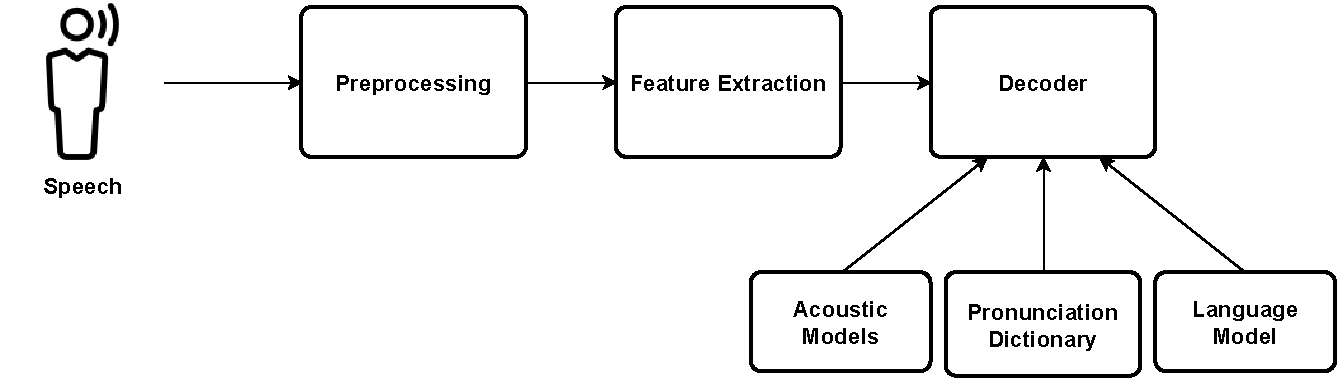
\includegraphics[width=\textwidth]{images/Hybrid ASR System.pdf} 
    \caption{A hybrid \acrshort{asr} system architecture}
    \label{fig:hyrid_asr_model}
  \end{center}
\end{figure}

In the \acrshort{hmm}-based architecture, the first step is preprocessing the speech signal to remove any unwanted noise and then convert to the required format for the next steps. Next, apply feature extraction methods to generate vectors which are used in the decoder. The decoder which consists of multiple models including acoustic models, pronunciation dictionary and language models then process the feature vectors from the previous stage.

\subsection{End to end speech recognition systems}
\label{section:e2easr}
In end to end speech recognition systems, a single model, usually based on deep learning, supersedes the hybrid \acrshort{asr} system stages. A deep learning model combined with an external language model can achieve higher performance than hybrid speech pipelines, while being simple to train. These systems rely on large neural networks and are trained on multiple \acrshort{gpu}s and thousands of hours of speech data. Since the system learns the whole task end-to-end, specialized components for capturing finer details of the speaker or other noise filtering components are not essential. On the contrary, previous experiments have shown that end to end models stand out in the cases where robustness is crucial. \cite{Hannun2014DeepRecognition}. 

\emph{In an end to end deep learning \acrshort{asr} system, we can achieve performance gains by improving three main components: model architecture, training data and computational infrastructure. The focus of this thesis is hence to increase the scale of data while making maximum use of the available computational resources, and trying out various experiments with different model architectures to analyse the effect it has on final performance of the system.}

\section{What are Deep Neural Networks?}
A deep neural network is a neural network with many hidden layers. Theoretically, deep neural networks can be trained to model non-linear models and functions for very high dimensional data. Traditionally, it was quite challenging to train deep neural networks, but there was a resurgence in the usage of deep neural networks in the previous decade, also in the field of speech recognition \cite{Dahl2012Context-DependentRecognition, Morgan2012DeepRecognition, Deng2013RECENTMICROSOFT, Hannun2014DeepRecognition}. 

One of the first deep neural network was a \acrfull{mlp}, which consists of an input layer, an output layer and a hidden layer. Figure \ref{fig:mlp} shows this architecture. 

\begin{figure}[ht]
  \begin{center}
    % below the size of the figure has been reduced for example
    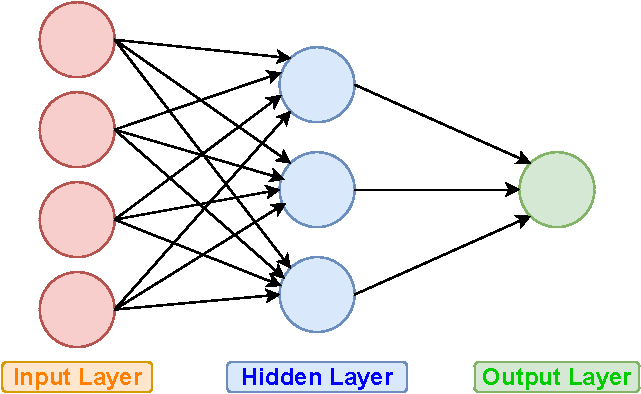
\includegraphics[width=\textwidth]{images/MLP.pdf} 
    \caption{An \acrshort{mlp} architecture}
    \label{fig:mlp}
  \end{center}
\end{figure}

Each layer of this network consists of multiple neurons, and each of these neurons can be represented using a vector, and all the neurons in a layer can then be represented using a weights matrix that determines how much a neuron should take part in the decision-making process. At each neuron, multiply the input signal with its corresponding weights and then added to have a weighed sum as the output of a layer. This can be represented as,

\[ z = w_1x_1 + w_2x_2 + .. + w_nx_n \]

In the above formula $z$ is the weighted sum output, $w$ is the weight, $x$ is an input and there are $n$ number of inputs. An activation function like tanh, sigmoid, ReLU, etc is applied to the weighted sum to get the output of the layer. 

The training process is a repetition of multiple such training batches until all the data is traversed once. This is referred to as an epoch. From the output, calculate the error by comparing it with the ground truth. This error is then backpropagated to all the previous layers to improve the network weights. Backpropagation requires an optimization algorithm like Stochastic Gradient Descent (SGD), Adaptive Momentum Estimation (Adam), etc. At the end of the training process, the main goal is to achieve high performance of the overall model by iteratively setting the right values for the weight matrices in each neuron.

\subsection {Recurrent Neural Networks}
A \acrfull{rnn} is a type of neural network that can predict a future state by taking the previous states as input. \cite{Graves2013SpeechNetworks} This network can be thought of as having memory because it considers the context of the input provided to determine the output state. \cite{Hagner2017RecurrentModel}

Figure \ref{fig:rnn} represents a basic unit of an \acrshort{rnn}. It consists of an extra synapse that loops back into itself. In practise, this means that each unit receives a new input and also receives the output from the previous units as an input.
\begin{figure}[ht]
  \begin{center}
    % below the size of the figure has been reduced for example
    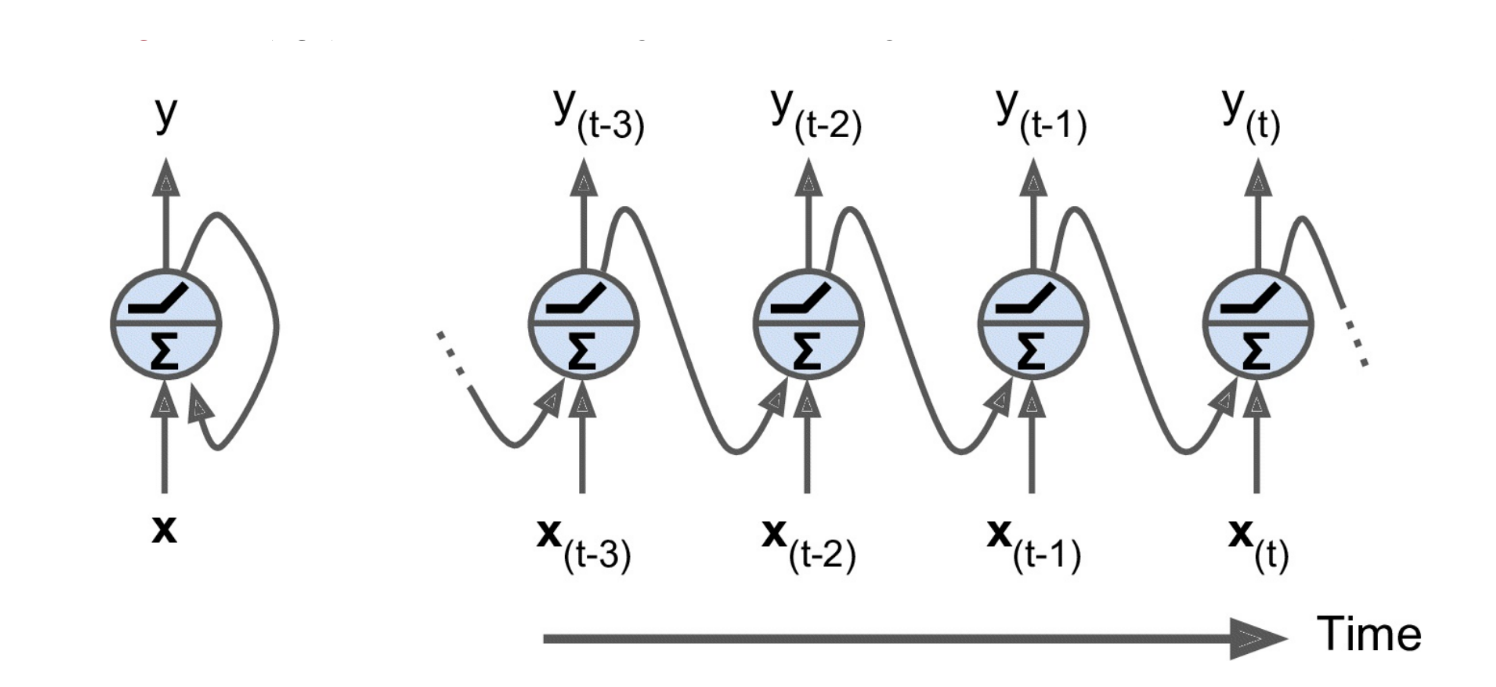
\includegraphics[width=\textwidth]{images/rnn.png} 
    \caption{A basic recurrent neural network cell and a way to visualize it
unrolling through time, from time step t-3 to t \cite{Hagner2017RecurrentModel}}
    \label{fig:rnn}
  \end{center}
\end{figure}

Consider an input series $\boldsymbol{x}=\left(x_{1}, \ldots, x_{T}\right)$, an \acrshort{rnn} calculates the hidden sequence $\boldsymbol{h}=\left(h_{1}, \ldots, h_{T}\right)$ and the output sequence $\boldsymbol{y}=$ $\left(y_{1}, \ldots, y_{T}\right)$ by looping the following equations from $t=1$ to $T$ :

$$
\begin{aligned}
&h_{t}=\mathcal{H}\left(w_{xh} x_{t}+w_{hh} h_{t-1}+b_{h}\right) \\
&y_{t}=w_{h y} h_{t}+b_{y}
\end{aligned}
$$

where the $w$ terms denote weight matrices, the $b$ terms denote bias vectors and $\mathcal{H}$ is the hidden layer function. \cite{Graves2013SpeechNetworks}

The drawback of an \acrshort{rnn} is that they use only the previous output to get the current context, but for speech recognition there is value to also utilize the future states too. A more advanced variation of \acrshort{rnn} is hence a \acrfull{brnn} \cite{Schuster1997BidirectionalNetworks} processing of the input happens in both directions using two hidden layers and then this used as input to a single output layer. 

\subsubsection{Long Short-term Memory (LSTM)}
By modifying the \acrshort{rnn} architecture, a \acrfull{lstm} cell \cite{Hochreiter1997LongMemory} passes another state vector to the next time step, along with the hidden state. The cell state variable enables the useful long term based information to be preserved because this is modified only when there is new information. To control the cell state, gates which multiply a signal that is 1 or 0 is used. Each gate has a weight matrix which are trained by iterating over the input data. The original work use two gates which are "input" gate, which control what information is essential and hence adds to the current state, and "output" gate which control what information needs to be written to the hidden state. More recently, a third gate called a "forget" gate controls deleting the unwanted information  from the cell state to stop cells growing in a boundless manner. \cite{Gers2000LearningLSTM}.

\begin{figure}[ht]
  \begin{center}
    % below the size of the figure has been reduced for example
    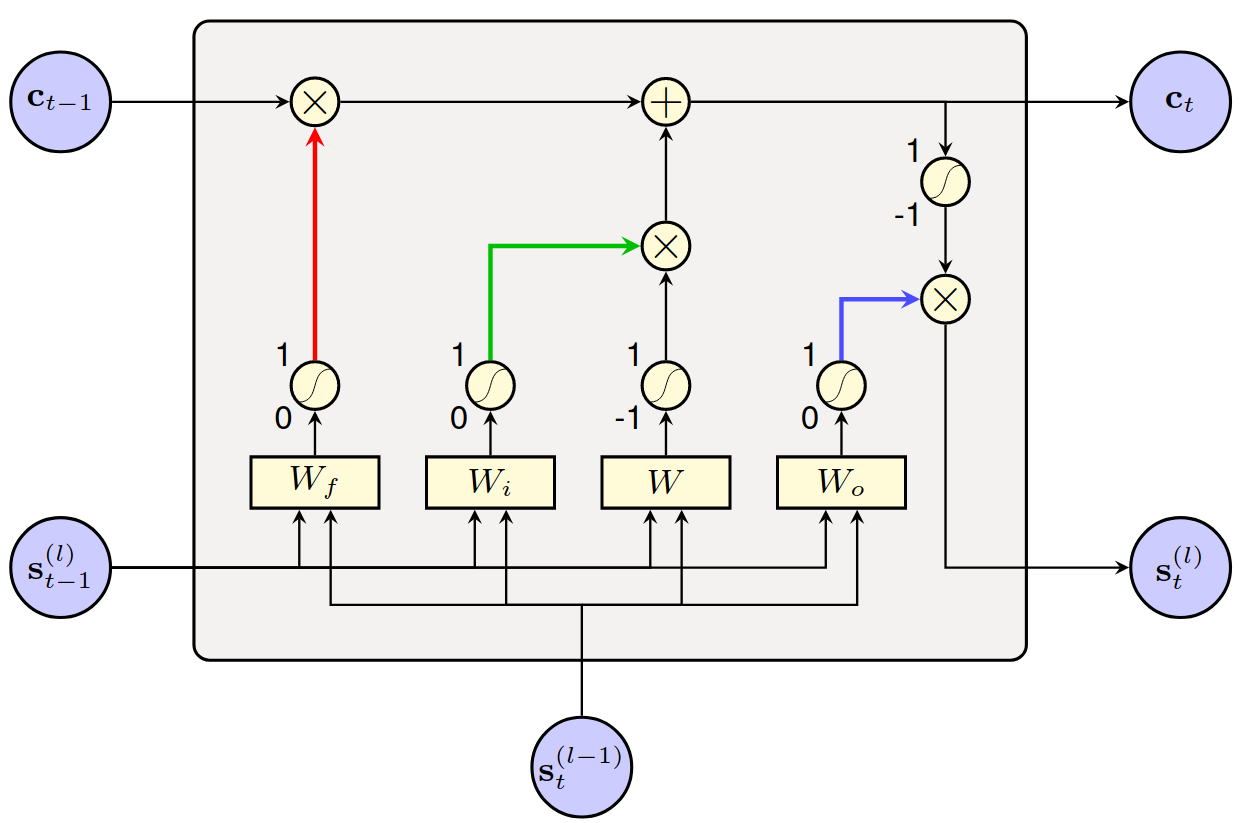
\includegraphics[width=\textwidth]{images/lstm.png} 
    \caption{A basic \acrshort{lstm} cell for a single time step \cite{Enarvi2018ModelingRecognition}}
    \label{fig:lstm}
  \end{center}
\end{figure}

Figure \ref{fig:lstm} shows the architecture of an \acrshort{lstm} layer with all the three gates. The three gates take in identical input, which also depends on how the definition of the network. In most cases, the input to \acrshort{lstm} cell is the combination of the hidden state of the previous time step ($c_{t-1}$) and the output of the previous layer. Each gate contains 2 weight matrices, one each for the two inputs, and a bias vector. (Figure \ref{fig:lstm} shows only a weight matrix per gate.) 


\subsection {Convolutional Neural Networks}
\acrfull{cnn} is a branch of neural networks, which are hierarchical in nature and rely on convolution operations to process input. \acrshort{cnn}s specialize in performing tasks like image classification, object detection, etc on images and videos. \acrshort{cnn}s perform well when spatial features are important to perform the given task. \cite{Krizhevsky2012ImageNetNetworks}

The architecture of a general \acrshort{cnn} is alternating layers of convolution with subsampling layers. \cite{Ciresan2011FlexibleClassification} The convolution layer has the parameters by size, kernel size, skipping factors and inter connections between the layers which are tuned to achieve high performance. Figure \ref{fig:cnn} shows the architecture of AlexNet, one of the most popular \acrshort{cnn}s for image classification. \cite{Krizhevsky2012ImageNetNetworks}. The architecture consists of convolutional layers altered with max pooling layers which act as sub sampling layers. The last layer of the network is using a fully connected layer to reduce the final dimensionality to match the required output shape.
\begin{figure}[ht]
  \begin{center}
    % below the size of the figure has been reduced for example
    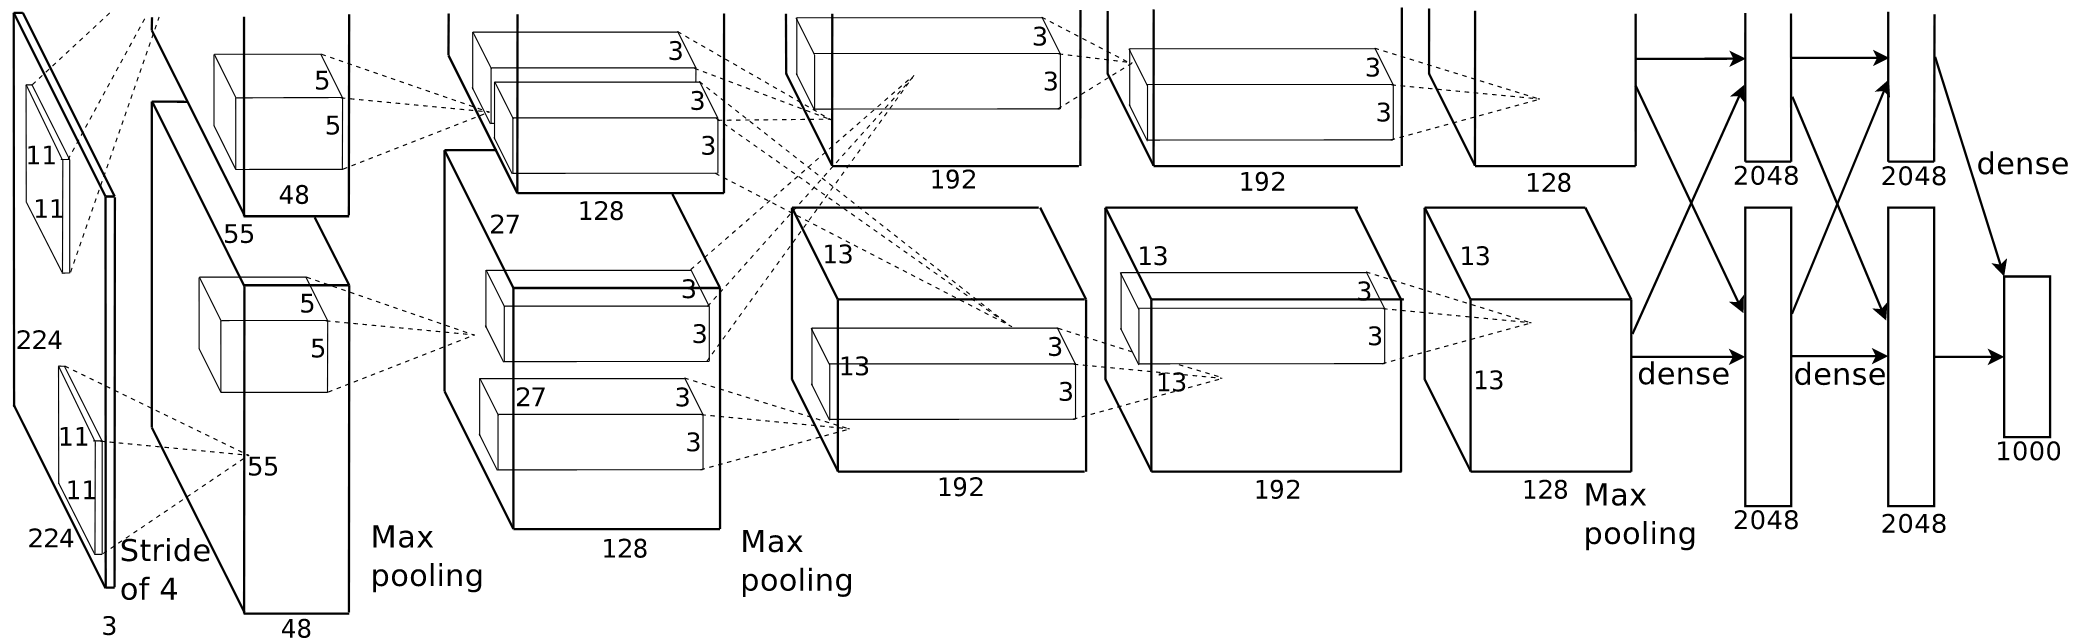
\includegraphics[width=\textwidth]{images/cnn.png} 
    \caption{AlexNet, a popular \acrshort{cnn} architecture  \cite{Krizhevsky2012ImageNetNetworks}}
    \label{fig:cnn}
  \end{center}
\end{figure}

More recently, convolutional neural networks have become popular for end to end speech recognition applications as well. \cite{Zhang2017VeryRecognition} The focus is on using convolutional layers along with a recurrent neural network. Unlike a typical \acrshort{rnn} with a fully connected layer, these networks replace it with a convolution layer because it is better at using the input topology to produce the required output. These neural networks which are a combination of convolutional layers and a recurrent network are hence termed as \emph{Convolutional Recurrent Deep Neural Network (CRDNN)}. 

\subsection {Listen, Attend and Spell (LAS)}
Encoder-decoder type architecture models have become extremely popular over the last few years and one of the variations in this branch of neural networks are the attention-based models. \cite{Vaswani2017AttentionNeed,  Prabhavalkar2017ARecognition} \acrfull{las} models are a combination of two sub-modules: the Listener module and the Attend-Speller module. The listener is an acoustic model encoder which converts the input signal to an embedding representation. The Attend-Speller module acts as a decoder module and takes the embeddings generated to produce a probability distribution for the output character sequences. \cite{Zhang2017VeryRecognition, Chan2016ListenRecognition}

\begin{figure}[ht]
  \begin{center}
    % below the size of the figure has been reduced for example
    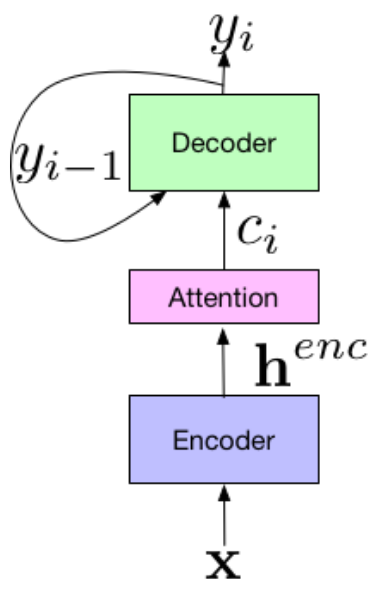
\includegraphics[width=0.3\textwidth]{images/las.png} 
    \caption{Architecture Diagram for a \acrshort{las} model  \cite{Chiu2017State-of-the-artModels}}
    \label{fig:las}
  \end{center}
\end{figure}

Figure \ref{fig:las} represents the architecture of a \acrshort{las} model with the Encoder as the Listen module and Attention and Decoder as the Attend-Speller module. The attention mechanism provides the context value. The below equations represents the functions in mathematical form.

$$
\begin{aligned}
\mathbf{h} &=\operatorname{Listen}(\mathbf{x}) \\
P\left(y_{i} \mid \mathbf{x}, y_{<i}\right) &=\text { AttendSpell }\left(y_{<i}, \mathbf{h}\right)
\end{aligned}
$$
where $ \mathbf{h}$ is the embedding representation, the output from the Listen module and $P\left(y_{i} \mid \mathbf{x}, y_{<i}\right)$ represents the probability of the output character based on the input signal and the previous output characters.

Let $\mathbf{x}=\left(x_{1}, \ldots, x_{T}\right)$ be the input sequence and $\mathrm{y}$ be the output sequence of characters. \acrshort{las} models produce for every character an output $y_{i}$ which is a conditional distribution based on the previously occurring characters $y_{<i}$ and the original signal $\mathrm{x}$ by making use of the chain rule for probabilities:

$$
P(\mathbf{y} \mid \mathbf{x})=\prod_{i} P\left(y_{i} \mid \mathbf{x}, y_{<i}\right)
$$

This defined the end to end nature of the \acrshort{las} models because it generates a probability distribution for the output characters sequence right from the input signal. 

\subsubsection{Connectionist Temporal Classification}
\label{section:ctc}
The connectionist temporal classification criteria is a way of training end-to-end models when the target sequence and the input sequence do not match exactly in length. It eliminates the need to align the target labels on a frame to frame basis with the input training signal. 

From the previous encoder-decoder architecture, the difference is that the conditional probability of the output character at each time step, the encoder output embeddings $\mathbf{h}$, are then fed to a softmax layer which considers the whole set of blank-augmented output symbols to predict a probability distribution output similar in nature to the typical encode decoder output.


\section{SpeechBrain Toolkit}
\label{section:sb}
Speech recognition have always been driven forward due to the critical role played by open-source toolkits such as HTK \cite{Young2002TheBook}, Kaldi \cite{Povey2011TheToolkit}, etc. More recently, general purpose deep learning frameworks like TensorFlow \cite{Abadi2016TensorFlow:Systems} and PyTorch \cite{Paszke2019PyTorch:Library} have become useful for speech recognition tasks and this has led to newer toolkits like ESPNet \cite{Watanabe2018ESPnet:Toolkit}. SpeechBrain \cite{Ravanelli2021SpeechBrain:Toolkit} is a toolkit designed to be flexible and used for multiple tasks to speed up research and development of speech related technologies.  SpeechBrain is a PyTorch-based toolkit and equipped to perform multiple tasks at once like recognize speech, understand its content, emotion, language, and speakers. 

\subsection{Brain class}
The SpeechBrain's core functionalities revolve around the \inlinecode{Brain} class, which defines a general training loop. The \inlinecode{Brain.fit()} method trains the models, and the Figure \ref{fig:brain} shows the basic components of the method. 

\begin{figure}[ht]
  \begin{center}
    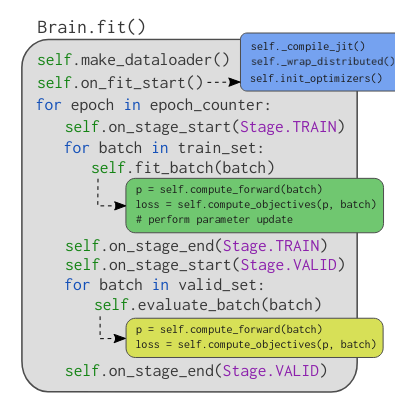
\includegraphics[width=0.5\textwidth]{images/brainclass.png} 
    \caption{\inlinecode{Brain.fit()} method illustration \cite{Ravanelli2021SpeechBrain:Toolkit}}
    \label{fig:brain}
  \end{center}
\end{figure}

Training of most \acrshort{dnn} models can be completed with a few lines of code. The Brain class also handles repetitive boilerplate code. It also takes care of validation, learning rate scheduling, recoverable fault tolerant checkpointing etc. Training a model happens through a python script and run from the command line with the combination of a configuration file: 
\begin{verbatim} python train.py train.yaml\end{verbatim}

\subsection{HyperPyYAML}
The configuration file is in YAML format which is human-readable and can be used to define the model architecture, the data files, the parameters of the model, hyperparameters for training and other characteristics of the pipeline. SpeechBrain utilities HyperPyYAML \footnote{speechbrain/HyperPyYAML:  Extensions  to  YAML  syntax  for  better python interaction. \href{https://github.com/speechbrain/HyperPyYAML}{https://github.com/speechbrain/HyperPyYAML} } which makes several extensions to the default YAML file format. The most important addition out of them is the easier object creation. An example:

\begin{verbatim}
epoch_counter: !new:speechbrain.utils.epoch_loop.EpochCounter
    limit: 100
\end{verbatim}

This tag with prefix \inlinecode{!new:} creates an instance of the specified class with an option to pass keyword arguments by using a mapping node like in the example above.

The next extension is the use of prefix, \inlinecode{!name} which simplifies the creation of an interface for specifying a function or class or other static Python entity. Below is an example using that.
\begin{verbatim}
opt_class: !name:torch.optim.Adam
    lr: !ref <lr>
\end{verbatim}
The prefix \inlinecode{!ref} is also an extension to the alias system used in YAML files. It takes keys in angles brackets and searched for the key within that YAML file. It can be used also for string interpolation, concatenation etc. It also has the \inlinecode{!include} prefix to import other YAML files to be used to reference in the current YAML file. This can be used to make the configuration files modular as well. 

\begin{verbatim}
dataset_parameters: !include:dataset.yaml
tokenizer_parameters: !include:tokenizer.yaml
\end{verbatim}

The last extension is the use of tuples. implicitly resolve any string starting with \inlinecode{(} and ending with \inlinecode{)} to a tuple.

\subsection{Other features}
SpeechBrain extends the PyTorch's data loading to help with speech data related challenges like handling variable length sequences and complicated data transformations. By leveraging PyTorch's \inlinecode{Dataset} and \inlinecode{DataLoader} classes, SpeechBrain enables on-the-fly data transformation (loading, augmentation, environment corruption, text processing, text encoding, feature extraction, etc) and can also be scaled to multiple parallel workers.

SpeechBrain also supports dynamic batching and multi \acrshort{gpu} training, which are discussed in detail in Chapter 4. This enables large-scale speech recognition tasks, which is the core of the work done in this thesis.  

\chapter{Large-Scale Speech Recognition}
\label{chapter:largescale}

\section{Overview}
End to end speech recognition models have millions of parameters and the architecture complexities make them highly data hungry \cite{Li2020OnRecognition}. Modern \acrshort{asr} systems have been designed to work in multiple domain and environment conditions, and this robustness is possible due to the usage of larger and larger datasets. One of the largest datasets is the 300,000 hours dataset from Google's research team. In their work, they have attempted to build a domain invariant speech recognition model using the large dataset\cite{Narayanan2019TowardTraining}. Other applications include multi-lingual \acrshort{asr} models \cite{Kannan2019Large-ScaleModel} and highly accurate domain-specific \acrshort{asr} models. These experiments showcase the ability of the \acrshort{asr} systems to perform at high levels by using more and more data. An observation from almost all of these works is that the researches are limited to an industrial domain and published by Google, Microsoft, etc who go through fewer budget constraints than other researchers in the domain of \acrshort{asr}. In the academic domain, the amount of research done in this direction is limited due to the resource constrains concerning \acrshort{gpu} resource, CPU resources, network communication availability of datasets, disk storage. 

\section{Scaling up training}
One of the major factors that have led to the rise in popularity of \acrshort{dnn}s, is due to the increase in the scale of data used to train them. There are three main dimensions in which this can be done. First is the magnitude of training data. The model performance can be improved by feeding more data to the deep neural network during training \cite{Hestness2017DEEPEMPIRICALLY}. The definition of a \emph{large-scale} dataset specific to speech recognition is ever-changing. For some context, a popular research in 2014 \cite{Hannun2014DeepRecognition}, used 5000 hours of training data and more recent research in 2020 \cite{Narayanan2019RECOGNIZINGMODELS}, researchers have used 300,000 hours of training data with random augmentation techniques for each epoch. Hence, we can observe that, In the previous 7 years, the training data used in researches has grown by multiple folds. Increasing the amount of high-quality training data hence is one of the unequivocal ways to improve performance of deep learning models. Hence, the practice of adding more and more training data is likely to continue through the next few years \cite{Mayer2020ScalableInfrastructures}. 


The second dimension is the scale of the infrastructure. The easily available parallel hardware, especially graphics processing units (\acrshort{gpu}s), has proven to be a great enabler to train \acrshort{dnn}s in shorter times than before \cite{Zhang2017Poseidon:Clusters}. This is also due to the reducing costs of hardware resources. Storing and handling data have become cheaper and easier \cite{Sayed2014ASecurity}. \acrshort{gpu} resources have become cheaper and more powerful, which have enabled researchers to use more data for training of deep neural networks \cite{Sayed2014ASecurity}. 

The third dimension is the size of the \acrshort{dnn} models, by increasing the width and depth of the models, \acrshort{dnn} models have increased in architectural complexity to achieve better results \cite{Dean2012LargeNetworks}. 

\section{Distributed Training}
Complex models trained on large datasets have shown good results \cite{Dean2012LargeNetworks}. Such huge training tasks can take models a few weeks or even months on a single \acrshort{gpu} to reach convergence. To increase the throughput of the training system, one of the straightforward  methods is by increasing the amount of compute resources, which include the number of \acrshort{gpu}s available. Distributed training is the method of training in a distributed infrastructure of multiple compute nodes, each with multiple \acrshort{gpu}s on it \cite{Langer2020DistributedPerspective}. 

This also brings with it many challenges. The first challenge is to use the computing resources efficiently. This should also go along with tight integration of hardware elements to improve the overall throughput of the system. Data transmissions across machines can be a common bottleneck when training a network. During training a deep neural network using SGD, the weights have to be synchronized across all the devices in use. As the amount of \acrshort{gpu}s in the system grows, the data transmission overhead also grows with it. These challenges require research at a confluence of both computing systems and deep learning training methods, and is receiving growing attention \cite{Xiao2018Gandiva:Learning, Mai2020KungFu:Adaptive, Chilimbi2014ProjectSystem, Cui2016GeePS:Server, Peng2018Optimus:Clusters}.

\subsection{Types of parallelism}
There are many ways to train deep learning models in parallel. The most common ones are discussed here, namely data and model parallelism.

\subsubsection{Model Parallelism}
In model parallelism, split the deep neural network into different devices and load a portion of the model on each device for training, as shown in Figure \ref{fig:modelparallel}. The device that holds the first layer receives the training data. Next, the data propagates through the rest of the forward pass on the device, and it passes the output to the device that holds the next layer of the DL model. During the backward pass, compute the gradients starting from the device that hold the output layer and then propagate the gradients to the devices backward till the device with the input layer. 

\begin{figure}[ht]
  \begin{center}
    % below the size of the figure has been reduced for example
    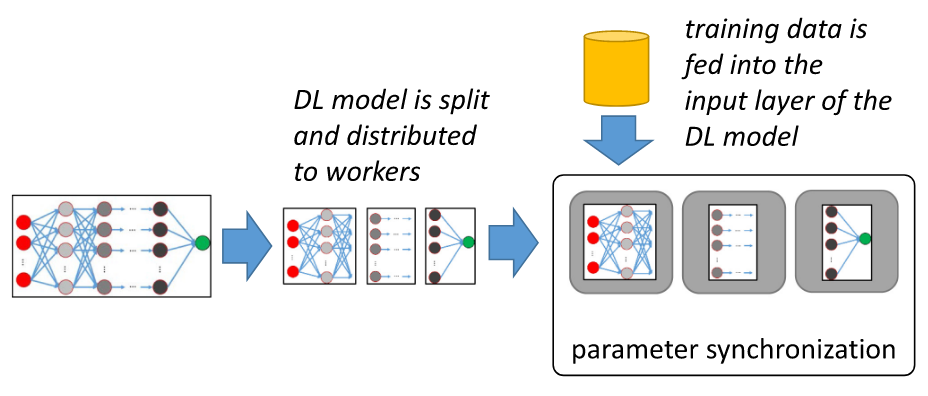
\includegraphics[width=\textwidth]{images/model parallelism.png} 
    \caption{Architecture Diagram of Model Parallelism  \cite{Mayer2020ScalableInfrastructures}}
    \label{fig:modelparallel}
  \end{center}
\end{figure}

The biggest challenge in model parallelism is to split the model into partitions such that the hardware efficiency on different devices is high during training \cite{Mayer2017ThePath}. In many cases, the best way is to empirically try out various permutations and measure the performance and keep the best permutation that has worked well. The second drawback is that model parallelism needs heavy communication between devices. A combined effect of these two challenges is that stalling may occur if models are hard to be split effectively to reduce the communication overloads and synchronization delays. Therefore, training speed might not increase linearly by increasing the number of parallel devices \cite{Mirhoseini2017DeviceLearning}.

The major benefit of the model parallelism is that it can accommodate huge deep learning networks, which cannot be stored on a single device (\acrshort{gpu}) to train them because the memory required to train them is split across multiple units. 

\subsubsection{Data Parallelism}
In data parallelism, copy the deep neural network into different devices and load an identical copy of the model on each device for training, as shown in Figure \ref{fig:dataparallel}. Split the data into the same number as the number of devices, and then data passes into the model replicas of the workers for training. Perform the training process on each chunk of the data that is assigned to the device to generate partial gradient updates of the model parameters. Once it is completed on all the processing units, the parameters are synchronized across all the devices \cite{Koliousis2019CROSSBOW:Servers}. 

\begin{figure}[ht]
  \begin{center}
    % below the size of the figure has been reduced for example
    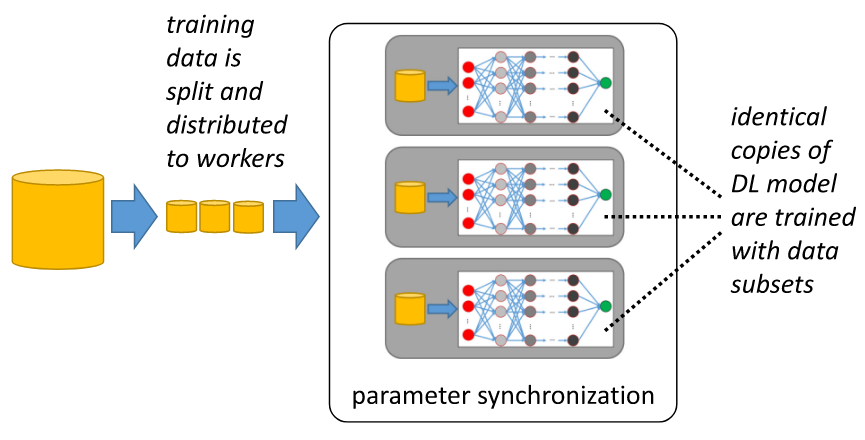
\includegraphics[width=\textwidth]{images/data parallelism.png} 
    \caption{Architecture Diagram of Data Parallelism  \cite{Mayer2020ScalableInfrastructures}}
    \label{fig:dataparallel}
  \end{center}
\end{figure}

Since each device processes a mini batch of data, the total batch size is the product of the mini batch with the number of \acrshort{gpu}s. This high data scale might lead to poor convergence. The other drawback is that ideally, the data that is split along the different workers needs to be identically distributed, so that the parameter updates by the different workers can be easily synchronized to get the overall model \cite{Jia2018BeyondNetworks}.

The major benefit of data parallelism is that it can be easily applied to most of the deep learning networks without much specific knowledge about the architecture of the model. It is highly scalable for the cases when the training is compute intensive but have relatively few parameters like \acrshort{rnn}s, \acrshort{cnn}s \cite{Krizhevsky2014OneNetworks}.


\subsection{Types of synchronization}
Due to the multiple nodes trying to update the model, the important question then becomes when to synchronize the parameters between the parallel workers. The main trade off is between managing training convergence and quality with synchronization cost to update all the models on the parallel workers. There are mainly two methods which are discussed here: synchronous and asynchronous methods.

\subsubsection{Synchronous}
The workers synchronize the weight updates after every batch of data processed. This is implemented in some of the first and prominent methods, like the \acrfull{bsp} \cite{Valiant1990AComputation} method, which is already available in popular data analytics platforms. The main advantage is that the model convergence is easier due to the strict nature of synchronization. However, this method is vulnerable to a situation where \emph{one} single worker stalls the entire training process, especially when the different nodes in the system are heterogeneous in nature \cite{Cipar2013SolvingStaleness}.

Synchronous training is already available in many open-source DL frameworks, such
as TensorFlow \cite{Abadi2016TensorFlow:Systems} and PyTorch \cite{Paszke2019PyTorch:Library}. Most ideally, it is best suited for a system where the nodes involved are homogeneous in nature with similar hardware configurations and hence stragglers are not a significant issue and there are minimal delays from communication.

\subsubsection{Asynchronous}
\label{section:hogwild}
The workers update the model parameters completely independent of other workers. Asynchronous training relies on the theoretical characteristic of SGD that the model convergence is robust to the random ordering of data. The model used by a worker at some point of time might be a stale model because there are no binding guarantees. This makes it difficult to assess model convergence using asynchronous training. However, the advantage is that the workers enjoy great levels of flexibility during training, hence avoiding the straggler problem that is faced in the synchronous method.

\emph{Hogwild} \cite{Niu2011HOGWILD:Descent} is one implementation of the asynchronous training of parallel SGD. Hogwild works by providing all the workers access to a shared memory space, which consists of the model parameters. This is completely lock-free, and hence seems dangerous because new model parameters from one worker can be completely overwritten by another worker without being used at all. Nevertheless, it has been shown that that since model updates are anyway sparse in nature when done sequentially, Hogwild also can achieve results similar to sequential training. This has been applied to large neural networks with good results \cite{Deyringer2017ParallelizationHogwild}. 


\subsection{Data Parallel Systems Architecture}
The architecture of the system defines \emph{how} the parameter synchronization among different workers happens in a data parallel system. There are three major considerations for the system architecture. Firstly, the architecture must be able to scale up to many parallel workers to update the DL model and also read the updated DL model. Secondly, the system needs to be configurable, that is, to be able to manage different parameter settings, etc. The third aspect is to be compatible with widely available inter process communication primitives.

\begin{figure}[ht]
  \begin{center}
    % below the size of the figure has been reduced for example
    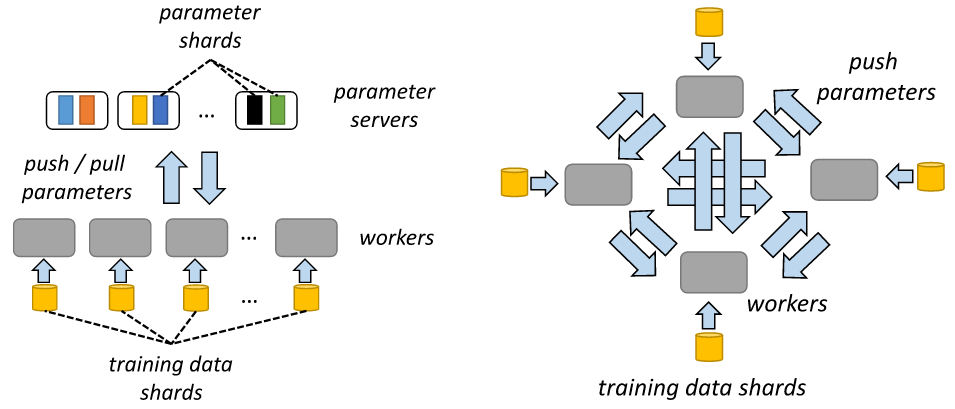
\includegraphics[width=\textwidth]{images/architecture_.png} 
    \caption{Diagram of centralized architecture on the left and decentralized architecture on the right.  \cite{Mayer2020ScalableInfrastructures}}
    \label{fig:arch}
  \end{center}
\end{figure}


\subsubsection{Centralized: Parameter Server}
Centralized architecture consists of a parameter server which is located (logically) in the centre and the worker nodes updates their computed gradients to the central server and all the workers then read the updated model to update their replicas of the model. This architecture is one of the most commonly used in a data parallel system. It is also common to use parameter shards to accelerate the process of communicating the parameter updates. Figure \ref{fig:arch} shows this architecture.

\subsubsection{Decentralized: allreduce Operation}
Decentralized architecture operates without a Parameter Server. The parameters synchronize directly by using an \inlinecode{allreduce} operation as shown in Figure \ref{fig:arch}. 

The major benefit of using a decentralized architecture is that there is no need for one node reserved for parameter server. There is also no single point of failure, and this makes it easier to manage fault tolerance. The major drawback of the decentralized architecture is that communication increases exponentially with the increase in number of workers. One way to avoid this is to use partial gradient updates. For each synchronization, every worker sends a partition of the gradients to every other worker. The communication costs now depend on the number of partitions \emph{and} also on the number of workers in the system. 

Both of these architectures, are widely adopted in leading open-source deep learning frameworks, however the decentralized architecture is the most suitable architecture for a system where there is a single node with multiple \acrshort{gpu}s attached because communication on the same node does not consume too much of resources. However, for multinode training, a centralized architecture works better\cite{Mayer2020ScalableInfrastructures}. 

A quick overview of practical considerations for different types of architecture, parallelism, and synchronization strategy can be accessed here \footnote{Distributed training with TensorFlow, TensorFlow Core. \href{https://www.tensorflow.org/guide/distributed\_training}{https://www.tensorflow.org /guide/distributed\_training} }. 

\section{Related works in large-scale ASR systems}
\label{section:largescale_related}
Large-scale speech recognition has had varying definitions even over the past few years. In 2014, authors applied data and model parallelism for training \acrshort{rnn}-based \acrshort{asr} models \cite{Hannun2014DeepRecognition}. They used 5000 hours of labelled data to build a multi-\acrshort{gpu} powered data-driven speech system which produced state-of-the-art results for that period of time. This solution was also quite robust to distortions and designed to work on both clear, conversational speech and also speech in noisy environments. The work also showed that with data parallelism on more than a few \acrshort{gpu}s, scaling up the overall batch size linearly with the number of \acrshort{gpu}s did not help with the model convergence rate.

More recently, research works from large enterprise companies have continued to focus on increasing the scale of training by multiple folds. Jinyu Li, et al. from Microsoft compare popular end to end speech recognition for large-scale \acrshort{asr} \cite{Li2020OnRecognition}. Authors consider an \acrshort{rnn} transducer, an Attention-based encoder decoder, and transformer architectures and train them with 65,000 hours of training data both for streaming mode and non-streaming modes. In their experiments, to maintain a fair comparison, they have fixed the overall number of parameters to a single limit of around 87M. Their results show that transformer models obtained the best \acrlong{wer}s (\acrshort{wer}) outperforming the other models by around 1\% \acrshort{wer}. They also report that pretraining works well even for large-scale tasks, compared to random initialization.

Google has also worked on increasing their scale of data used for their experiments. In 2019, researches have published their work on building a domain invariant speech recognition model, using large amounts of data from multiple domains to train a single model that work across different applications, sampling rates, audio codecs and formats, and  noise conditions \cite{Narayanan2019TowardTraining}. They claim that their model can adapt to an entirely new domain with as little as one tenth of data compared to that required for a model trained from scratch. This helps to develop speech recognition models for practically any environment with less amount of data. Since then, recent Google research has used datasets that are a huge 300,000 hours in size \cite{Narayanan2019RECOGNIZINGMODELS}. The dataset consists of data from voice search, far field use cases, telephone speech, and audio from YouTube videos. This nature of multi-domain data is again useful for inter-domain speech recognition applications. They also compare the impact of increasing data diversity in improving performance of the models. The authors assess how best to use multi domain data when different proportions of data are available from different domains. They try training models using equal probability from different domain and ignore the relative distribution of data among the domains. From their experiments, this usually tended to overfit the domains that had lesser data. Hence, the overall conclusion was to sample the data from all domain with the probability proportional to the total number of utterances in the domain. Overall, they report that using multi domain data and in large scales improved the output performance of the model significantly.

The previously discussed datasets are not available in public domain, and this has been one of the major issues for developing models for large-scale speech recognition jobs in academic backgrounds. Recent efforts \cite{Galvez2021TheUsage, Pratap2020MLS:Research} have been to create such a publicly available dataset that can be used in academic research. The People's Speech dataset \cite{Galvez2021TheUsage} is a free to download dataset with 31400 hours with more data continuously added. The data, collected by scraping the internet for appropriately licensed audio data with transcriptions. The data collected is diverse in nature, with varying sampling rates, background noise and different forms of speech. There are a few problems with this dataset, as the authors state that there is no defined measure if there are duplicates in the dataset because the dataset's creation is by crawling the internet, it is possible that some data appears twice in the dataset. This also means that creating test sets with no overlap with the training set is challenging. 

Multilingual LibriSpeech (MLS) \cite{Pratap2020MLS:Research} dataset is the first attempt to create a large scale multilingual dataset. It has a total of 32,000 hours of English data and 4,500 hours of data from 7 other languages. The dataset is entirely audiobooks, with  transcriptions downloaded from the internet and then aligned with the audio. This dataset can be used for both speech recognition and text to speech applications since the audio is quite clean with minimal to zero background noise. 

Common Voice \cite{Ardila2020CommonCorpus} is a crowd-sourced multilingual dataset that is mainly focused to propel automatic speech recognition tasks. This dataset is easily scalable for any language because community efforts drives both data collection and data validation. At the time of writing this report, the common voice dataset has 12,500 hours of labelled data \footnote{Common Voice. \href{https://commonvoice.mozilla.org/en}{https://commonvoice.mozilla.org/en}}. For many of the languages in the common voice dataset, it is the only publicly available dataset source for speech recognition tasks. Users can record audio by reading out sentences or phrases that are shown to them through common voice's app or website. The text used in common voice comes mainly from Wikipedia articles. For data validation, a maximum of three volunteers listen to an audio clip and the clip is valid as soon as two votes are positive.

\section{Summary}
It is apparent from industry-based research that there are huge improvements and advantages to be gained from increasing the dataset size used for training the models. There is a lot of work done in this direction to scale up the amount of publicly available speech data that can be used for academic research. \emph{Hence, it is time for researchers in academic field to be well-prepared to scale up training by multiple folds in the near future. The aim of this thesis is to act as a guidebook for scaling up training in multiple steps of the training process.} The next chapters discuss the best methods to store data, loading of data, training using multi-\acrshort{gpu}s, training using multiple processes and reporting performance.



\chapter{Implementation}
\label{chapter:methods}

\section{Overview}
In this chapter, we start of by discussing the dataset used and what makes the dataset unique in Section \ref{section:bizspeech}. Then, we look at how to make the data usable for an \acrshort{asr} application with steps like forced alignment and audio normalization in Section \ref{section:dataprep}. Next, we go over the details for training the acoustic encoder decoder model used in Section \ref{section:attention_train}. Lastly, we explore the distributed methodologies used and discuss the practical choices taken when using those methods in Section \ref{section:di}



\section{Business Speech (BizSpeech) Dataset}
\label{section:bizspeech}
As mentioned in the Section \ref{section:largescale_related}, there are not many datasets which are available publicly for training speech recognition systems at a scale of around tens of thousands of hours. This section introduces Business Speech dataset, which has been used for all the experiments in this thesis. 

Business speech dataset consists of conference calls, which are corporate disclosure and brokerage event information. It can be accessed through a paid licence here\footnote{Company Events Coverage, StreetEvents, Refinitiv. \href{https://www.refinitiv.com/en/financial-data/company-data/company-events-coverage}{https://www.refinitiv.com/en/ financial-data/company-data/company-events-coverage}}. Refinitiv also provides transcriptions, call summaries and other metadata like date and PermID, which is the ID number for the firm. This ID can further be used to link to many more metadata information from other datasets like the officers and directors dataset\footnote{Officers and Directors data, Refinitiv \href{https://www.refinitiv.com/en/financial-data/company-data/officers-and-director-search}{https://www.refinitiv.com/en/financial-data/ company-data/officers-and-director-search}} which provides information about the firm's financials, personnel involved etc. The audio and transcripts can be accessed via APIs and also via the Eikon software\footnote{Eikon Financial Analysis \& Trading Software, Refinitiv \href{https://www.refinitiv.com/en/products/eikon-trading-software}{https://www.refinitiv.com/ en/products/eikon-trading-software}} \cite{August2011ThomsonEikon}. Figure \ref{fig:eikon} shows a snapshot of the software in use.

\begin{figure}[ht]
  \begin{center}
    % below the size of the figure has been reduced for example
    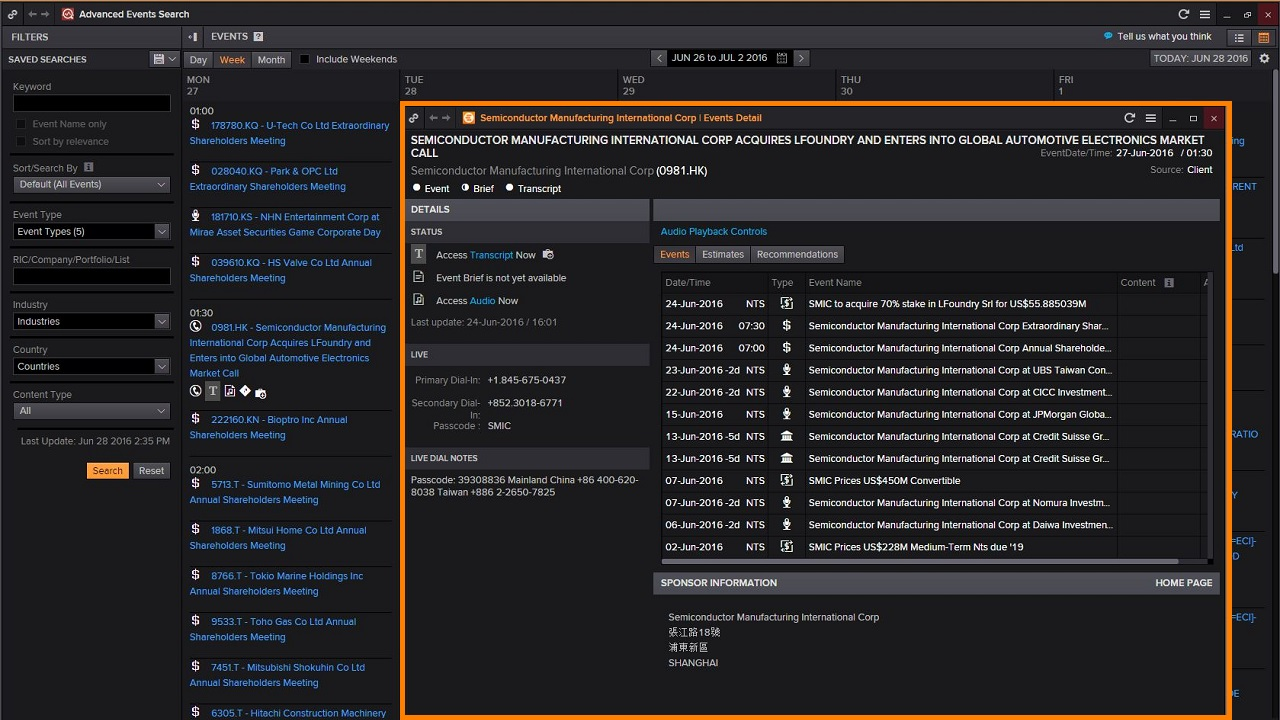
\includegraphics[width=\textwidth]{images/company-events-coverage-eikon.jpg} 
    \caption{Conference call event information in Eikon.}
    \label{fig:eikon}
  \end{center}
\end{figure}

The dataset which is used for the experiments consist of 24,793 conference calls held by 6,131 firms all over the world. All the calls are in English language. Approximately 80\% of the firms are from English-speaking countries. Earnings calls pertaining to fiscal year 2017 contribute to 68\% of the dataset, 22\% are from 2016 and 5\% each is from 2015 and 2018. 
The conference calls are one-hour long conversations with the initial part of the call consists of a presentation about the firm's financials in the previous period and the rest of the call is a question and answer session with journalists and other analysts. Hence, the dataset has different types of speech, prepared one-sided speech is in the first half of the audio and the rest are more conversational in nature. The speech is mostly in the sphere of finance and business and consists of a lot of jargon from this domain. The dataset has different speech from different English accents. An analysis of the companies' metadata show that the dataset consists of conference calls of companies from 76 countries. Out of the 24793 events, 4822 (around 20\%) are from non-native English-speaking countries. Even among the native English-speaking countries, there is a wide distribution of events between the USA, UK, Australia, New Zealand, etc.

Since there are no publicly available results on this dataset for the task of automatic speech recognition, a portion of it was processed using popular cloud speech to text services to analyse the complexity of the dataset. Azure's\footnote{Speech to Text, Audio to Text Translation, Microsoft Azure \href{https://azure.microsoft.com/en-us/services/cognitive-services/speech-to-text/}{https://azure.microsoft .com/en-us/services/cognitive-services/speech-to-text/}} speech to text service and Google's\footnote{Speech-to-Text: Automatic Speech Recognition, Google Cloud \href{https://cloud.google.com/speech-to-text/}{https://cloud.google. com/speech-to-text/}} speech to text services analysed around 2000 randomly sampled utterances from the BizSpeech dataset. The word error rates (WER) on the two services were 19.74\% and 21.9\% on Azure and Google, respectively. Furthermore, on analysing the word error rates based on the nationality of the companies, from Figure \ref{fig:wer_cloud} we can observe that on Google, there is a drop of 32.7\% in WER and in Azure, the drop is 36.5\% from native to non-native utterances which shows that even the most generalized models can suffer with different speaking conditions. 

\begin{figure}[ht]
  \begin{center}
    % below the size of the figure has been reduced for example
    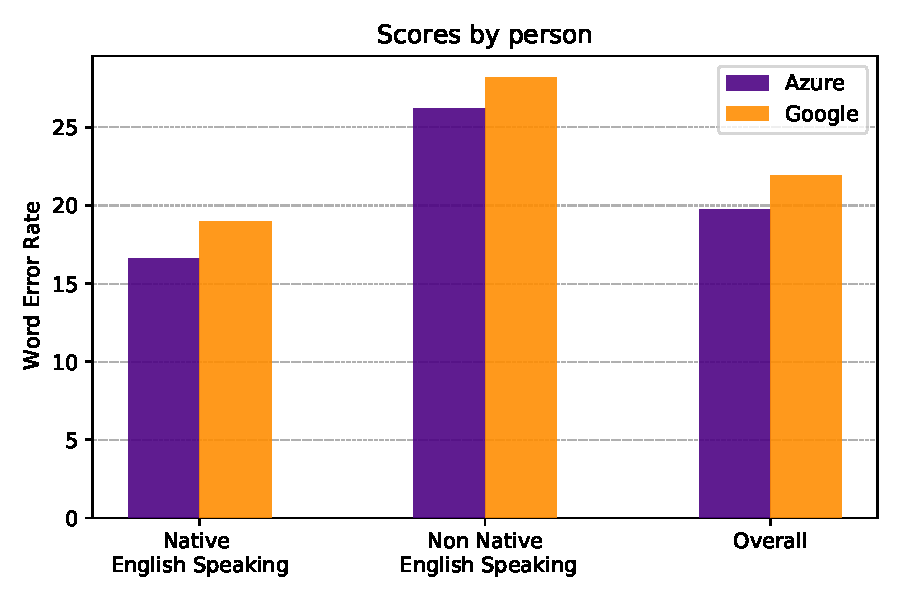
\includegraphics[width=0.8\textwidth]{images/wer_cloud.pdf} 
    \caption{Word Error Rate on Google's and Azure's cloud services.}
    \label{fig:wer_cloud}
  \end{center}
\end{figure}


The main advantage of this dataset is that it is quite a large dataset and includes various speech styles and accents. The drawback of the dataset is that the speech is from a single domain and from a specific field, which might mean that the models trained on this dataset might not be useful for general speech recognition tasks.

The transcript in the dataset consists of text with punctuations and with standard capitalization applied. The dataset consists of non-standard text, like abbreviations, random characters to represent word fillers (like ah, eh, oh.) and many abbreviations and named entities. The phrase "operator instructions" is used in the transcript very frequently to denote that the conference operator is giving out instructions pertaining to the call, and the actual phrase is not present in the audio at all. These inconsistencies (examples shown in Table \ref{table:examples}) make the dataset harder to train and since the size of the dataset is large, it is hard to know where and what other inconsistencies are present in the dataset. 

\begin{table}[ht]
\begin{tabular}{ l p{9.6cm} c c }

 \hline
 \multicolumn{2}{c}{\textbf{Punctuation}} \\
 \hline
 \textbf{Transcript:} & \verb|[..] with the short-term dynamics?| \\ 
 \textbf{Verbatim:} & \verb|[..] with the short term dynamics| \\
 \textbf{Model output:} & \verb|[..] with the short-term dynamics?| \\
 \hline\hline

 \multicolumn{2}{c}{\textbf{Capitalization}} \\
 \hline
 \textbf{Transcript:} & \verb|Hi. This is Andy.| \\ 
 \textbf{Verbatim:} & \verb|hi this is andy| \\
 \textbf{Model output:} & \verb|Hi, this is Andy.| \\
 \hline\hline
 
 \multicolumn{2}{c}{\textbf{Abbreviations \& Named Entities}} \\
 \hline
 \textbf{Transcript:} & \verb|[..] a question from Andrew Porteous, HSBC.| \\ 
 \textbf{Verbatim:} & \verb|[..] a question from andrew porteous h s b c| \\
 \textbf{Model output:} & \verb|[..] a question from Andrew Porteous, HSBC.| \\
 \hline\hline
 
 \multicolumn{2}{c}{\textbf{Random characters}} \\
 \hline
 \textbf{Transcript:} & \verb|[..] things are -- [theoretically], good| \\ 
 \textbf{Verbatim:} & \verb|[..] things are eh theoretically good| \\
 \textbf{Model output:} & \verb|[..] things -- theoretically, good| \\
 \hline\hline
 
 \multicolumn{2}{c}{\textbf{Transcript inconsistencies}} \\
 \hline
 \textbf{Transcript:} & \verb|Operator Instructions| \\ 
 \textbf{Verbatim:} & \verb|welcome to the petit home q one results call| \\
 \textbf{Model output:} & \verb|Welcome to the Petit Home Q1 Results Call.|\\
 \hline\hline
\end{tabular}
\caption{\label{table:examples}Examples of non-standard text in the dataset. For each example, we show the ground truth transcript, the verbatim transcript, which is exact audible speech from the audio file, and the ASR model output, which is the output of our trained end to end speech to text model.}
\end{table}


\section{Data Preparation}
\label{section:dataprep}
After downloading the dataset, training \acrshort{asr} models still requires a few preprocessing steps. This section explains these preprocessing steps in more detail. 

The audio recordings in the BizSpeech dataset, are a mix of MP3 and WAV files which have varying sampling rates between 8 kHz, 16 kHz and 32 kHz. We convert all the audio to WAV format with 16 kHz sampling rate to maintain uniformity across the whole dataset.

\subsection{Forced Alignment}
Even though they have transcripts for the speech, most of them lack timestamps for the utterances or are inaccurate. The audio files are also around 1 hour long in length, and hence it would be impossible to use the data for training \acrshort{asr} models without finer and accurate timestamps for the sentences. 

\begin{figure}[ht]
  \begin{center}
    % below the size of the figure has been reduced for example
    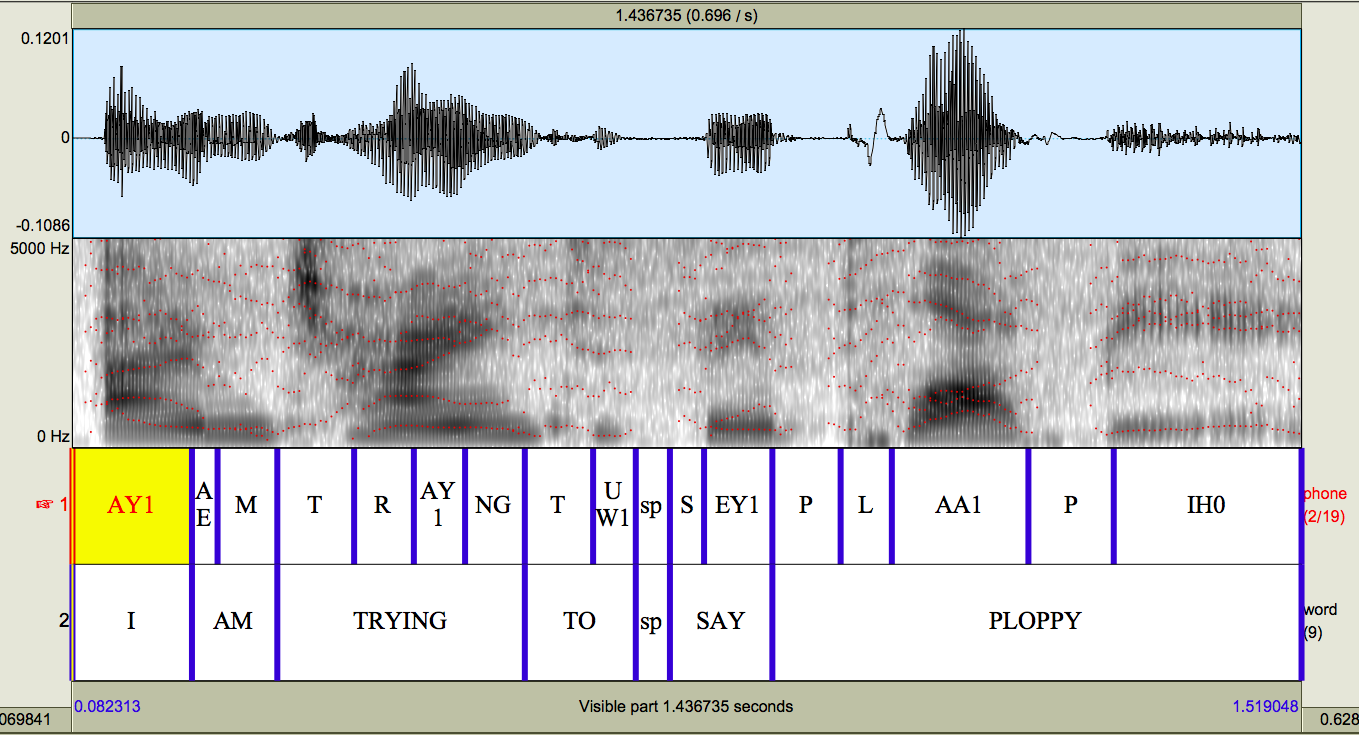
\includegraphics[width=0.8\textwidth]{images/ploppy.png} 
    \caption{Result of forced alignment for an example input. \cite{Yuan2008SPEAKERCORPUS}}
    \label{fig:p2fa}
  \end{center}
\end{figure}

We use forced alignment to generate accurate alignment of speech with the textual data. Forced alignment helps to align linguistic units (e.g., phoneme or words) with the corresponding audio file. It requires an audio file with transcriptions as input, and it outputs the text with word level time-aligned data. We use the P2FA for Python 3\footnote{Penn Phonetics Lab Forced Aligner Toolkit (P2FA) for Python3, \href{https://github.com/jaekookang/p2fa\_py3}{https://github.com/ jaekookang/p2fa\_py3}} tool, which is a \acrshort{hmm} forced aligner based on P2FA \cite{Yuan2008SPEAKERCORPUS} to generate alignments. The aligner works by using a HTK \cite{Young2002TheBook} based acoustic model along with a pronunciation dictionary. The tool generates the transcript's phoneme representation, and then the acoustic model generates accurate time-aligned output. An example of this can be seen in Figure \ref{fig:p2fa}.

As mentioned in their work, the errors for the successful alignments are around 50ms. A risk of using forced aligner is that it always tries to generate some sort of alignment. When any sorts of inconsistencies are present with the text and audio, for example, a missing word in the transcript, can deceive the tool for the whole file's alignment and the tool fails. It is difficult to automatically detect these cases and a human test is expensive, especially at the scale of the BizSpeech dataset. Due to this issue, \emph{the usable data from the 24,793 audio hours for training \acrshort{asr} model is finally 19973 hours with close to 9 million utterances with a composition of 52,484 speakers.}

\subsection{Data Loading Performance}
Now that accurate time alignments are available for the dataset, we split the large audio files into smaller files such that each audio split has one sentence in it. Each one of these splits is linguistically a sentence, and we label them as an individual utterance and store as a WAV file. We store the text for the utterance in a JSON file along with a few metadata fields, with a unique utterance ID as the filename for both the audio clip and the JSON file. 


Each utterance length ranges from one second up to 60 seconds. Figure \ref{fig:utt_dist} shows the distribution of the utterance length for the whole dataset. We can see that most of the utterances are around the 6-second length. Since, the utterances are small in relative to the overall size of the dataset (close to 20,000 hours) there are about 9 million audio files and 9 million JSON files to be loaded for every training run. This becomes highly inefficient\footnote{Small files, Aalto scientific computing \href{https://scicomp.aalto.fi/triton/usage/smallfiles/}{https://scicomp.aalto.fi/triton/usage/ smallfiles/}} and will lead to problems on opening too many files on the training node. The size of the dataset is also around 5 TB, which makes it hard to store on a single disk storage. Hence, we cannot depend on storing the data on the local SSD drive. All these problems lead to extremely high usage of disk storage, disk I/O usage, network costs (especially for multi node training), and high CPU usage to access and read a high number of files. 


\begin{figure}[ht]
  \begin{center}
    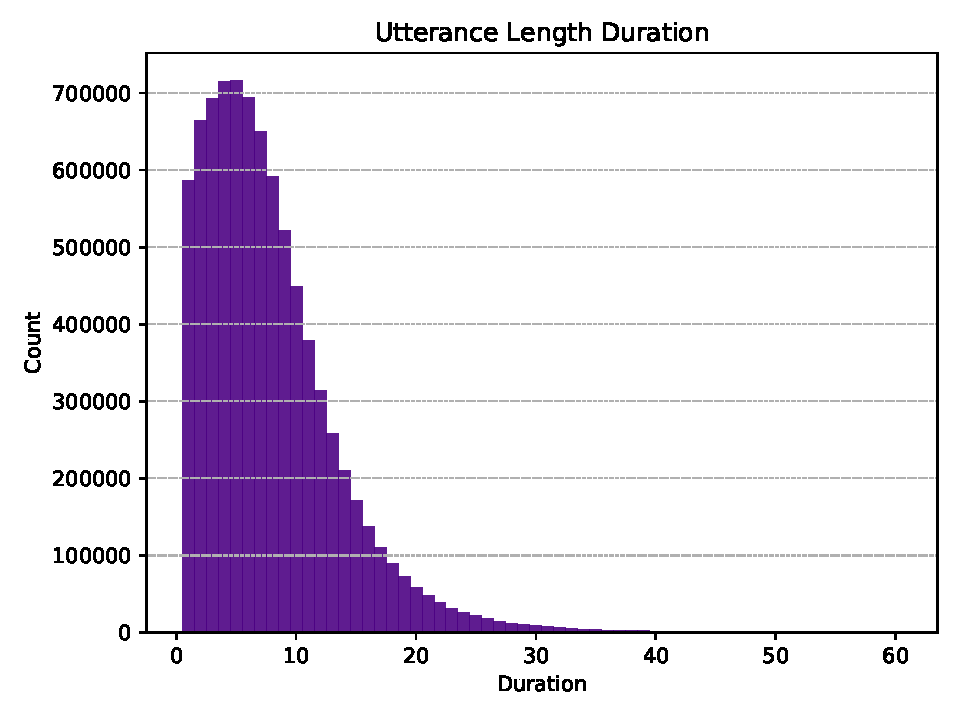
\includegraphics[width=\textwidth]{images/duration_distribution.pdf} 
    \caption{Utterance Duration Distribution for BizSpeech Dataset}
    \label{fig:utt_dist}
  \end{center}
\end{figure}

Hence, we use WebDataset\footnote{webdataset/webdataset: A high-performance Python based I/O system for large (and small) deep learning problems, with strong support for PyTorch. \href{https://github.com/webdataset/webdataset/}{https://github.com/ webdataset/webdataset/}}\cite{Aizman2019HighLearning}, a PyTorch Dataset (\inlinecode{IterableDataset}\footnote{torch.utils.data, PyTorch 1.9.0 documentation \href{https://pytorch.org/docs/stable/data.html}{https://pytorch.org/docs/stable/data .html}}) implementation which provides high efficiency access to data stored in TAR\footnote{GNU tar 1.34: Basic Tar Format \href{https://www.gnu.org/software/tar/manual/html_node/Standard.html}{https://www.gnu.org/software/tar/manual/html\_ node/Standard.html}} archives. This uses only sequential/streaming data access, which brings substantial performance advantage. Figure \ref{fig:seq} shows, on the left side, a file-based access to resources and on the right side, an illustration of sequential based access to resources. We can see from the illustration that sequential data access is much faster and requires much lesser communication. Typically, a ten-fold increase in performance can be seen during I/O operations\cite{Aizman2019HighLearning} for a single node setup with sequential access. This enables large-scale training. Because, it supports basic TAR archives the other advantage is that it becomes easy to create, manage and distribute the data for deep learning training. Since, TAR can be compressed using gzip\footnote{gzip, Wikipedia \href{https://en.wikipedia.org/wiki/Gzip}{https://en.wikipedia.org/wiki/Gzip}} and this is supported directly by webdataset and this helps to save storage space as well. Webdataset can also be set up to use sharding. Sharding helps achieve high throughput using parallel I/O with multiprocess enabled tasks like data loading, preprocessing, etc. This. We specify the shards as a list of files to webdataset, or they can be written using the brace notation. For example, \inlinecode{bizspeech-shard-\{000000..003000\}.tar} means there are 3000 shards. When used with a standard Torch \inlinecode{DataLoader}, this will perform parallel I/O and preprocessing. 


\begin{figure}[ht]
  \begin{center}
    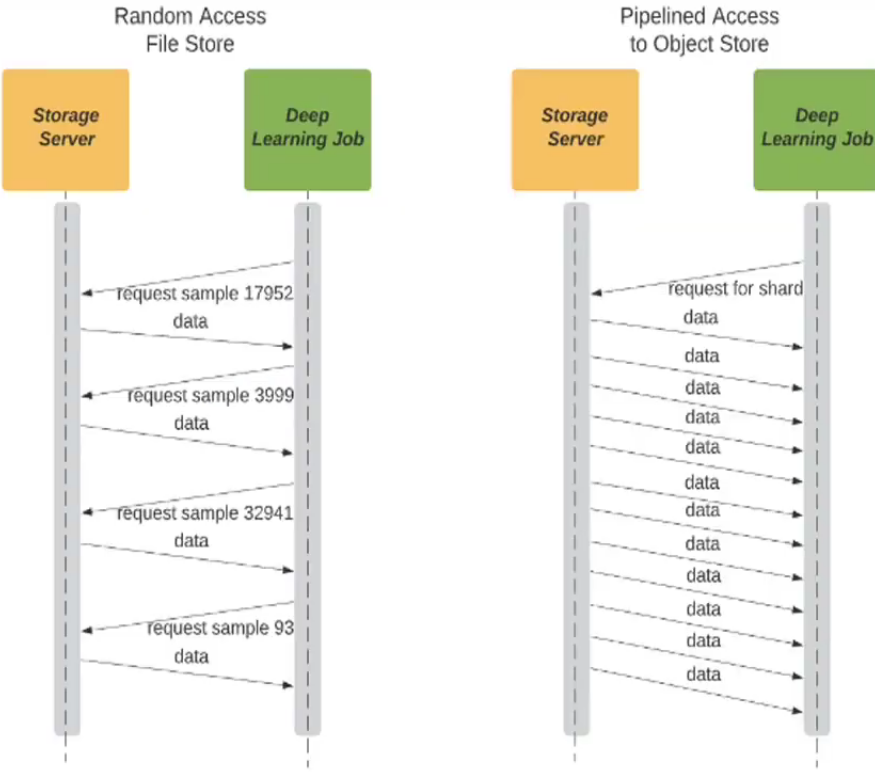
\includegraphics[width=0.7\textwidth]{images/sequential.png} 
    \caption{File-based Access vs Sequential Data Access \cite{Aizman2019HighLearning}}
    \label{fig:seq}
  \end{center}
\end{figure}

\emph{We convert the BizSpeech dataset  to compressed tar to enable usage of webdataset. Split the dataset into 3000 shards, with each shard containing about 700 MB of data after compression, totalling at around 2.1TB storage footprint. This dataset is now ready to be used for training ASR models efficiently. Empirically, speed-up after using webdataset with a single process was around 7-8 fold during training a small subset of 80 hours of the dataset. It becomes very difficult practically to store and test the file-based mechanism to measure the throughput difference for very large-scale experiments. For all the large-scale experiments of order more than 200 hours, we use a configuration of 2-4 worker processes per GPU with sharding and randomization enabled.}

\section{Training Attention based Encoder-Decoder model}
\label{section:attention_train}
For training a speech to text model on BizSpeech dataset, we use SpeechBrain (introduced in Section \ref{section:sb}). SpeechBrain provides recipes which are designed and further optimized for particular datasets. Considering the scale of experiments, we use the LibriSpeech recipe\footnote{speechbrain/recipes/LibriSpeech/ASR/seq2seq \href{https://github.com/speechbrain/speechbrain/tree/develop/recipes/LibriSpeech/ASR/seq2seq}{https://github.com/speechbrain/spee chbrain/tree/develop/recipes/LibriSpeech/ASR/seq2seq}} as a starting point for our experiments. After data loading and preprocessing to parse the audio and transcript text, we generate features from the audio signal. We use logarithmic, mel-based, filter banks 
\cite{Vetterli1992WaveletsDesign} with  0-8000 Hz frequency and the processing happens on-the-fly with data loading. These steps can be parallelized easily by enabling multiprocessing to increase the number of available workers loading the data. From the recipe, we disable the Language Model for our experiments because the focus is on scaling up the training of speech to text and not necessarily to make the model the most accurate one. The final model and configuration used is given in the Appendix \ref{chapter:model-architecture}. We use the negative log likelihood loss function along with the CTC loss (described in Section \ref{section:ctc}) for the initial 15 epochs. 

\subsection{Dynamic Batching}
\label{section:dynbatch}
A problem in automatic speech recognition is when batching up the utterances for training, the varying lengths of utterances means that the shorter utterances have to be padded up to the length of the longest utterance in the batch. Depending on the ordering of the utterances, the batches of data used for training could be high in sparsity due to padding. Because the ordering of training data is usually random, a fixed batch size can be inefficient when the utterances are short. To counter this, we sort the speech data in length to make the \acrshort{gpu} usage more efficient. However, this may affect the model convergence based on the type of ordering used. To solve these problems, SpeechBrain uses dynamic batch data loader where it reads the audio samples to the memory buffer. It then clusters the audio samples based on length and then generates batches of audio samples from similar length utterances, hence avoiding the inefficiencies in data loading due to padding issues. 

\subsection{\emph{Epoch} with dynamic batching}
The data is in random order, and since the data loading workers access the shards asynchronously, it is difficult to keep track of exact epochs (exact epoch here refers to each data sample used exactly once per epoch). Hence, we drop the "one sample per epoch" standard, and instead use sampling with replacement where we draw a sample completely randomly. Previous experiments have shown that sampling by replacement is as good as or in some cases better than one sample per epoch strategy \cite{Recht2012BeneathConsequences, Nielsen2015NeuralLearning}.Tracking the training progress generally involves observing the loss values and accuracy metrics of a validation step after every epoch of training, and since with the newer approach, traditional "epochs" are inconsequential, we track the number of updates to the model. We run the validation step after every 5000 updates to the model. Henceforth, \emph{epoch} refers to 5000 updates to the model and this is used to track training progress using validation loss and validation \acrshort{wer}.

\section{Distributed training}
\label{section:di}
We use two different methods of Multi-GPU training, \acrfull{ddp} is a synchronous, decentralized and as the name suggests, a data-parallel method. Hogwild is an asynchronous, data parallel method. 

\subsection{Synchronous Training}
We use PyTorch's distributed data parallel method to train our model \cite{Li2020PyTorchTraining}. This method enables training in distributed systems by passing gradients before the optimizer step is invoked. This ensures that all model replica parameters are updated using the same gradients, and thus the replicas stay synchronized across all the iterations. Hence, this can be equated to accumulating gradient across multiple batches of data on a single GPU. PyTorch uses \inlinecode{AllReduce} operation which is supported by primitive inter process communication libraries like NCCL\footnote{NVIDIA Collective Communications Library (NCCL), NVIDIA Developer \href{https://developer.nvidia.com/nccl}{https:// developer.nvidia.com/nccl}}, MPI\footnote{Open MPI: Open-Source High-Performance Computing \href{https://www.open-mpi.org/}{https://www.open-mpi.org/}}, etc. The \inlinecode{AllReduce} operation expects a tensor of the same size from all of its participant process and applies a given arithmetic operation, and sends back the output tensor to all the processes involved. It is through this operation that DDP becomes a synchronous method because \inlinecode{AllReduce}  waits until all processes join for a particular iteration, and each individual process waits for the output from \inlinecode{AllReduce} before it moves to the next iteration. More specifically, for implementing DDP for our models, SpeechBrain wraps the models with a \inlinecode{DistributedDataParallel} module from PyTorch. The data loader explained in Section \ref{section:dataprep} scales without any modifications required for a distributed training use-case. We use different processes (can be $>1$ process per replica as well) to load data for the different model replicas.

\subsection{Asynchronous Training}
We implement Hogwild \cite{Niu2011HOGWILD:Descent}, discussed in Section \ref{section:hogwild}. We discuss the parallel processing steps in more details here. We assume a shared parameter model across $p$ processors. The parameters are denoted by $x$ and each process accesses $x$ and can update $x$ because $x$ is stored in shared memory. To update the weights with an update $a$, there is no locking system enforced, so any process can perform the following operation on the shared memory.

$$
x_{v} \leftarrow x_{v}+a
$$

Once the training starts, each processor follows the pseudocode provided in Algorithm \ref{alg:hogwild}. It loads the current state of the model, $x_e$. Let $G_{e}(x)$ denote a gradient of the function $f_{e}$, as in standard \acrshort{sgd}, for a data point $e$ sampled randomly from the dataset, $E$. $\gamma$ is the step size and controls the magnitude of the gradient update. The gradients are updated directly without blocking the other processes.

\RestyleAlgo{ruled}

\begin{algorithm}
\caption{Hogwild algorithm for each process.}\label{alg:hogwild}
\While{}{
    Sample $e$ uniformly at random from $E$
    
    Read current state $x_e$ and evaluate $G_e(x)$
    
    $x_{v} \leftarrow x_{e}-\gamma G_{e}(x)$
}
\end{algorithm}

Once updated, the loop continues with its next iteration by loading new data and loading newer parameters from the shared memory. Since there is no blocking of the model parameters, sometimes  it could so happen that an update of the parameters is overwritten without being used by any processors at all. Results from \cite{Niu2011HOGWILD:Descent} however show that the training can benefit from the non-blocking nature of the training procedure. This is mainly because of the robustness of \acrshort{sgd} to the random ordering of updates to the parameters. \acrshort{sgd} is invariant to the data order and hence to the order in which the updates to the model are received.



\chapter{Evaluation}
\label{chapter:evaluation}

You have done your work, but that's\footnote{By the way, do \emph{not} use
shorthands like this in your text! It is not professional! Always write out all
the words: ``that is''.} not enough. 

You also need to evaluate how well your implementation works.  The
nature of the evaluation depends on your problem, your method, and
your implementation that are all described in the thesis before this
chapter.  If you have created a program for exact-text matching, then
you measure how long it takes for your implementation to search for
different patterns, and compare it against the implementation that was
used before.  If you have designed a process for managing software
projects, you perhaps interview people working with a waterfall-style
management process, have them adapt your management process, and
interview them again after they have worked with your process for some
time. See what's changed.

The important thing is that you can evaluate your success somehow.
Remember that you do not have to succeed in making something spectacular; a
total implementation failure may still give grounds for a very good master's
thesis---if you can analyze what went wrong and what should have been
done. 

 

 
\chapter{Discussion}
\label{chapter:discussion}


\section{Future Work}

\subsection{Dataset related work}
The dataset used is large and this has enabled all the experiments that we have conducted, but the dataset is not without its drawbacks and future work can be done to address some of these inconsistencies. There are phrases like "Operator Instructions" which are discussed in Section \ref{section:bizspeech} which are wrong transcriptions of what is being said in the audio, and this only came to our attention in the later stages of our experiments. Although some preprocessing steps were taken, the dataset needs more thorough cleaning to remove utterances like the above example from the dataset, which can then lead to better models.

The dataset can also be used for a wide variety of other applications like named entity recognition when properly tagged and in other domains to infer business related results based on the speech in the earnings calls. Also, due to the varied nature of the speakers, it can also be filtered and used to train models which are designed to work with a diverse set of speakers.  

\subsection{Further ASR Experiments}
Changing the model architecture can be tried and experiments involving scaling both model and data can be analysed and the correlation between the two scaling methods can be studied in detail. This could help establish a practical formula which can help researchers decide what minimum amount of data will be required to train models with certain number of parameters. Experiments can also focus on deeper and wider layers in the \acrshort{aed} model. Other architectures like transformers\cite{Vaswani2017AttentionNeed}, conformers\cite{Gulati2020Conformer:Recognition} can be explored for large-scale \acrshort{asr} experiments. This could be easy to extend using the same pipeline, but by replacing the model architecture with various other models.

With more time, we would have liked to tune hyperparameters for each type of training and analyse the best word error rates from the different techniques. Currently, the results indicate that methods that work with large batch sizes have fared well and models seem to struggle when batch size is reduced. It will be interesting to see if this holds even after varying the other hyperparameters like the learning rate, adding a learning rate scheduler, different optimizers etc. In all our experiments, the acoustic models are trained end-to-end with punctuations, capitalizations and other special characters. This is one of the biggest unknown in the experiments, about how the model would vary if it was trained with the normalized text instead. 

\subsection{Evaluation Methods}
For evaluating the models, we choose the best validation word error rate checkpoint as the final model to be used with the test set. However, in many cases we observed a sharp decline between the validation word error rates and the test word error rates even when both the sets are unseen and sampled randomly. This can be avoided by techniques like averaging checkpoints over multiple epochs, which have competitive error rates. This method should be used in the future experiments.
\chapter{Conclusions}
\label{chapter:conclusions}

Time to wrap it up!  Write down the most important findings from your
work.  Like the introduction, this chapter is not very long.  One to
two (never over three) pages might be a good limit. Still, the chapter
gives the background, goals, content, and the findings. However, all that
should already be in the previous chapters. This is just a summary (as
are the abstract and the introduction).

For making PDF/A version requested by the Aalto Library, open the end result pdf file in Acrobat and store it as PDF/A. Then verify the result (everything should be fine, at least as PDF/A-2b version works).

Congratulations, your thesis is ready and it looks beautiful!


% Load the bibliographic references
% ------------------------------------------------------------------
% You can use several .bib files:
% \bibliography{thesis_sources,ietf_sources}

\clearpage
\addcontentsline{toc}{chapter}{Abbreviations and Acronyms}
\chapter*{Abbreviations and Acronyms}

% The longtable environment should break the table properly to multiple pages, 
% if needed

\noindent
\begin{longtable}{@{}p{0.25\textwidth}p{0.7\textwidth}@{}}
ASR & Automatic Speech Recognition \\
DNN & Deep Neural Networks \\ 
GPU & Graphics Processing Unit \\

\end{longtable}

\clearpage
\addcontentsline{toc}{chapter}{Bibliography}
\bibliography{sources}


% Appendices go here
% ------------------------------------------------------------------
% If you do not have appendices, comment out the following lines
\appendix
\chapter{Model architecture}
\label{chapter:model-architecture}

\section*{Encoder Architecture}

\begin{verbatim}
CRDNN(
  (CNN): Sequential(
    (block_0): CNN_Block(
      (conv_1): Conv2d(
        (conv): Conv2d(1, 128, kernel_size=(3, 3), 
                        stride=(1, 1))
      )
      (norm_1): LayerNorm(
        (norm): LayerNorm((40, 128), eps=1e-05, 
                            elementwise_affine=True)
      )
      (act_1): LeakyReLU(negative_slope=0.01)
      (conv_2): Conv2d(
        (conv): Conv2d(128, 128, kernel_size=(3, 3), 
                        stride=(1, 1))
      )
      (norm_2): LayerNorm(
        (norm): LayerNorm((40, 128), eps=1e-05, 
                        elementwise_affine=True)
      )
      (act_2): LeakyReLU(negative_slope=0.01)
      (pooling): Pooling1d(
        (pool_layer): MaxPool2d(kernel_size=(1, 2), 
                            stride=(1, 2), padding=(0, 0), 
                            dilation=(1, 1), ceil_mode=False)
      )
      (drop): Dropout2d(
        (drop): Dropout2d(p=0.15, inplace=False)
      )
    )
    (block_1): CNN_Block(
      (conv_1): Conv2d(
        (conv): Conv2d(128, 256, kernel_size=(3, 3), 
                        stride=(1, 1))
      )
      (norm_1): LayerNorm(
        (norm): LayerNorm((20, 256), 
                            eps=1e-05, elementwise_affine=True)
      )
      (act_1): LeakyReLU(negative_slope=0.01)
      (conv_2): Conv2d(
        (conv): Conv2d(256, 256, kernel_size=(3, 3), 
                        stride=(1, 1))
      )
      (norm_2): LayerNorm(
        (norm): LayerNorm((20, 256), eps=1e-05, 
                        elementwise_affine=True)
      )
      (act_2): LeakyReLU(negative_slope=0.01)
      (pooling): Pooling1d(
        (pool_layer): MaxPool2d(kernel_size=(1, 2), 
                            stride=(1, 2), padding=(0, 0), 
                            dilation=(1, 1), ceil_mode=False)
      )
      (drop): Dropout2d(
        (drop): Dropout2d(p=0.15, inplace=False)
      )
    )
  )
  (time_pooling): Pooling1d(
    (pool_layer): MaxPool2d(kernel_size=(1, 4), 
                    stride=(1, 4), padding=(0, 0), 
                    dilation=(1, 1), ceil_mode=False)
  )
  (RNN): LSTM(
    (rnn): LSTM(2560, 512, num_layers=4, 
            batch_first=True, dropout=0.15, bidirectional=True)
  )
  (DNN): Sequential(
    (block_0): DNN_Block(
      (linear): Linear(
        (w): Linear(in_features=1024, 
                    out_features=256, bias=True)
      )
      (norm): BatchNorm1d(
        (norm): BatchNorm1d(256, eps=1e-05, 
                    momentum=0.1, affine=True, 
                    track_running_stats=True)
      )
      (act): LeakyReLU(negative_slope=0.01)
      (dropout): Dropout(p=0.15, inplace=False)
    )
    (block_1): DNN_Block(
      (linear): Linear(
        (w): Linear(in_features=256, out_features=256, 
                    bias=True)
      )
      (norm): BatchNorm1d(
        (norm): BatchNorm1d(256, eps=1e-05, 
                        momentum=0.1, affine=True, 
                        track_running_stats=True)
      )
      (act): LeakyReLU(negative_slope=0.01)
      (dropout): Dropout(p=0.15, inplace=False)
    )
  )
)
\end{verbatim}


\section*{Decoder Architecture}

\begin{verbatim}
AttentionalRNNDecoder(
  (proj): Linear(in_features=1024, out_features=512, bias=True)
  (attn): LocationAwareAttention(
    (mlp_enc): Linear(in_features=256, 
                    out_features=512, bias=True)
    (mlp_dec): Linear(in_features=512,
                    out_features=512, bias=True)
    (mlp_attn): Linear(in_features=512, 
                    out_features=1, bias=False)
    (conv_loc): Conv1d(1, 10, kernel_size=(201,), 
                    stride=(1,), padding=(100,), 
                    bias=False)
    (mlp_loc): Linear(in_features=10, 
                    out_features=512, bias=True)
    (mlp_out): Linear(in_features=256, 
                    out_features=512, bias=True)
    (softmax): Softmax(dim=-1)
  )
  (drop): Dropout(p=0.15, inplace=False)
  (rnn): GRUCell(
    (rnn_cells): ModuleList(
      (0): GRUCell(640, 512)
    )
    (dropout_layers): ModuleList()
  )
)

\end{verbatim}


\chapter{Configuration Files}
\label{chapter:hyparam}

\section*{dataset.yaml}
\begin{verbatim}
seed: 98585
__set_seed: !apply:torch.manual_seed [!ref <seed>]
dataset_seed: 26000

output_folder: !ref runs/<seed>
save_folder: !ref <output_folder>/save
local_dataset_folder: !ref /m/triton/scratch/
    biz/bizspeech/ASR_Datasets/<dataset_seed>/datasets 

# Path where data manifest files will be stored
train_annotation: !ref <local_dataset_folder>/train.json
valid_annotation: !ref <local_dataset_folder>/val.json
test_annotation: !ref <local_dataset_folder>/train.json

# Webdataset Parameters
use_wds: True
number_of_shards: 3000
#shard_maxcount: 10000
shardfiles_pattern: !ref <local_dataset_folder>/
    bizspeech_shard-%06d.tar.gz
use_compression: True
train_shards: (0, 2994)
val_shards: (2994, 2997)
test_shards: (2997, 3000)

# Audio Resampling and convert to single channel
sample_rate: 16000
preprocess_audio: !new:speechbrain.dataio.
            preprocess.AudioNormalizer
    sample_rate: !ref <sample_rate>
    mix: avg-to-mono

# Set up folders for reading from and writing to
data_folder: /scratch/biz/bizspeech/MEDIA 
hours_reqd: 26000
nonnative: 0.3
qna: 0.6
sorting: random # ascending
non_CEO_utt: True
strict_included: False
utterance_duration_limit: 1000 # in seconds
audio_filetype: wav
trainValTest: (1,0)
\end{verbatim}

\section*{tokenizer.yaml}
\begin{verbatim}
dataset: !include:dataset.yaml

# Tokenizer parameters
token_type: bpe  # ["unigram", "bpe", "char"]
token_output: 5000  # index(blank/eos/bos/unk) = 0
character_coverage: 1.0
annotation_read: txt # field to read

# Tokenizer train object
tokenizer_train: !name:speechbrain.
    tokenizers.SentencePiece.SentencePiece
   model_dir: !ref <dataset[save_folder]>
   vocab_size: !ref <token_output>
   annotation_train: !ref <dataset[train_annotation]>
   annotation_read: !ref <annotation_read>
   model_type: !ref <token_type> # ["unigram", "bpe", "char"]
   character_coverage: !ref <character_coverage>
   annotation_list_to_check:
     - !ref <dataset[train_annotation]>
     - !ref <dataset[valid_annotation]>
   annotation_format: json
   
\end{verbatim}

\section*{train.yaml}
\begin{verbatim}
dataset: !include:dataset_200.yaml
tokenizer_params: !include:tokenizer.yaml

train_WER_required: False
wer_file: !ref <dataset[output_folder]>/wer.txt
wer_file_p: !ref <dataset[output_folder]>/wer_p.txt
train_log: !ref <dataset[output_folder]>/train_log.txt
tensorboard_dir: !ref runs/tensorboard_log/<dataset[seed]>

tokenizer: !new:sentencepiece.SentencePieceProcessor

pretrainer: !new:speechbrain.
    utils.parameter_transfer.Pretrainer
   collect_in: !ref <dataset[save_folder]>
   loadables:
      tokenizer: !ref <tokenizer>
      #model: !ref <model>
   paths:
      tokenizer: !ref <dataset[save_folder]>/
        <tokenizer_params[token_output]>_
        <tokenizer_params[token_type]>.model

gradient_accumulation: False
subbatches_count_for_grad_acc: 4
require_native_wer: False
wer_native_file: !ref <dataset[output_folder]>
    /wer_native.txt
wer_nonnative_file: !ref <dataset[output_folder]>
    /wer_nonnative.txt
libri:
    test_on_librispeech: False
    data_folder: librispeech
    test_csv:
        - !ref <libri[data_folder]>/test-clean.csv
        - !ref <libri[data_folder]>/test-other.csv
    tokenizer: !ref <tokenizer>
    bos_index: 0
    eos_index: 0
    test_dataloader_opts:
        batch_size: 8
        num_workers: 1
    
train_logger: !new:speechbrain.
    utils.train_logger.FileTrainLogger
    save_file: !ref <train_log>

log_to_tensorboard: True
tensorboard_logger: !new:speechbrain.
    utils.train_logger.TensorboardLogger
    save_dir: !ref <tensorboard_dir>

# Training parameters
number_of_epochs: 50
number_of_ctc_epochs: 15
batch_size: 8
lr: 0.0001
ctc_weight: 0.5
ckpt_interval_minutes: 15 
label_smoothing: 0.1

# Dataloader options
train_dataloader_opts:    
    batch_size: null
    num_workers: 8
valid_dataloader_opts:
    batch_size: null
    num_workers: 1
test_dataloader_opts:
    batch_size: null
    num_workers: 1

use_dynamic_batch_size: True
looped_nominal_epoch: 5000
dynamic_batch_kwargs:  
    len_key: "sig"
    min_sample_len: 15999 
    # 1s * 16000
    max_sample_len: 960000
     # 60s * 16000 (Sample rate)
    sampler_kwargs:
        target_batch_numel: 2880000  
        # 180s * 16000 (Sample rate)
        max_batch_numel: 3840000 
        # 240s * 16000 (Sample rate)


# Feature parameters
n_fft: 400
n_mels: 40

# Model parameters
activation: !name:torch.nn.LeakyReLU
dropout: 0.15
cnn_blocks: 2
cnn_channels: (128, 256)
inter_layer_pooling_size: (2, 2)
cnn_kernelsize: (3, 3)
time_pooling_size: 4
rnn_class: !name:speechbrain.nnet.RNN.LSTM
rnn_layers: 4
rnn_neurons: 512
rnn_bidirectional: True
dnn_blocks: 2
dnn_neurons: 256
emb_size: 128
dec_neurons: 512
output_neurons: 5000  
blank_index: 0
bos_index: 0
eos_index: 0
unk_index: 0

# Decoding parameters
min_decode_ratio: 0.0
max_decode_ratio: 1.0
valid_beam_size: 80
#test_beam_size: 80
eos_threshold: 1.5
using_max_attn_shift: True
max_attn_shift: 240
lm_weight: 0.50
ctc_weight_decode: 0.0
coverage_penalty: 1.5
temperature: 1.25

epoch_counter: !new:speechbrain.
    utils.epoch_loop.EpochCounter
    limit: !ref <number_of_epochs>



# Feature extraction
compute_features: !new:speechbrain.
    lobes.features.Fbank
    sample_rate: !ref <dataset[sample_rate]>
    n_fft: !ref <n_fft>
    n_mels: !ref <n_mels>

# Feature normalization (mean and std)
normalize: !new:speechbrain.
    processing.features.InputNormalization
    
encoder: !new:speechbrain.
        lobes.models.CRDNN.CRDNN
    input_shape: [null, null, !ref <n_mels>]
    activation: !ref <activation>
    dropout: !ref <dropout>
    cnn_blocks: !ref <cnn_blocks>
    cnn_channels: !ref <cnn_channels>
    cnn_kernelsize: !ref <cnn_kernelsize>
    inter_layer_pooling_size: 
        !ref <inter_layer_pooling_size>
    time_pooling: True
    using_2d_pooling: False
    time_pooling_size: !ref <time_pooling_size>
    rnn_class: !ref <rnn_class>
    rnn_layers: !ref <rnn_layers>
    rnn_neurons: !ref <rnn_neurons>
    rnn_bidirectional: !ref <rnn_bidirectional>
    rnn_re_init: True
    dnn_blocks: !ref <dnn_blocks>
    dnn_neurons: !ref <dnn_neurons>
    use_rnnp: False

embedding: !new:speechbrain.
    nnet.embedding.Embedding
    num_embeddings: !ref <output_neurons>
    embedding_dim: !ref <emb_size>

# Attention-based RNN decoder.
decoder: !new:speechbrain.
    nnet.RNN.AttentionalRNNDecoder
    enc_dim: !ref <dnn_neurons>
    input_size: !ref <emb_size>
    rnn_type: gru
    attn_type: location
    hidden_size: !ref <dec_neurons>
    attn_dim: 512
    num_layers: 1
    scaling: 1.0
    channels: 10
    kernel_size: 100
    re_init: True
    dropout: !ref <dropout>

# Linear transformation on the top of the encoder.
ctc_lin: !new:speechbrain.nnet.linear.Linear
    input_size: !ref <dnn_neurons>
    n_neurons: !ref <output_neurons>

# Linear transformation on the top of the decoder.
seq_lin: !new:speechbrain.nnet.linear.Linear
    input_size: !ref <dec_neurons>
    n_neurons: !ref <output_neurons>

# Final softmax (for log posteriors computation).
log_softmax: !new:speechbrain.nnet.activations.Softmax
    apply_log: True

# Cost definition for the CTC part.
ctc_cost: !name:speechbrain.nnet.losses.ctc_loss
    blank_index: !ref <blank_index>


modules:
    encoder: !ref <encoder>
    embedding: !ref <embedding>
    decoder: !ref <decoder>
    ctc_lin: !ref <ctc_lin>
    seq_lin: !ref <seq_lin>
    normalize: !ref <normalize>

model: !new:torch.nn.ModuleList
    - - !ref <encoder>
      - !ref <embedding>
      - !ref <decoder>
      - !ref <ctc_lin>
      - !ref <seq_lin>

valid_search: !new:speechbrain.
        decoders.S2SRNNGreedySearcher
    embedding: !ref <embedding>
    decoder: !ref <decoder>
    linear: !ref <seq_lin>
    bos_index: !ref <bos_index>
    eos_index: !ref <eos_index>
    min_decode_ratio: !ref <min_decode_ratio>
    max_decode_ratio: !ref <max_decode_ratio>

test_search: !new:speechbrain.
        decoders.S2SRNNGreedySearcher
    embedding: !ref <embedding>
    decoder: !ref <decoder>
    linear: !ref <seq_lin>
    bos_index: !ref <bos_index>
    eos_index: !ref <eos_index>
    min_decode_ratio: !ref <min_decode_ratio>
    max_decode_ratio: !ref <max_decode_ratio>

opt_class: !name:torch.optim.Adam
    lr: !ref <lr>

error_rate_computer: !name:speechbrain.
    utils.metric_stats.ErrorRateStats

cer_computer: !name:speechbrain.
    utils.metric_stats.ErrorRateStats
    split_tokens: True

checkpointer: !new:speechbrain.
    utils.checkpoints.Checkpointer
    checkpoints_dir: !ref <dataset[save_folder]>
    recoverables:
        model: !ref <model>
        scheduler: !ref <lr_annealing>
        normalizer: !ref <normalize>
\end{verbatim}




% End of document!
% ------------------------------------------------------------------
% The LastPage package automatically places a label on the last page.
% That works better than placing a label here manually, because the
% label might not go to the actual last page, if LaTeX needs to place
% floats (that is, figures, tables, and such) to the end of the 
% document.
\end{document}
